% define document type (i.e., template. Here: A4 APA manuscript with 12pt font)
\documentclass[man, 12pt, a4paper, mask]{apa7}

% change margins (e.g., for margin comments):
%\usepackage{geometry}
% \geometry{
% a4paper,
% marginparwidth=30mm,
% right=50mm,
%}

% add packages
\usepackage[american]{babel}
\usepackage[utf8]{inputenc}
\usepackage{csquotes}
\usepackage{hyperref}
\usepackage[style=apa, sortcites=true, sorting=nyt, backend=biber, natbib=true, uniquename=false, uniquelist=false, useprefix=true]{biblatex}
\usepackage{authblk}
\usepackage{graphicx}
\usepackage{setspace,caption}
\usepackage{subcaption}
\usepackage{enumitem}
\usepackage{lipsum}
\usepackage{soul}
\usepackage{xcolor}
\usepackage{fourier}
\usepackage{stackengine}
\usepackage{scalerel}
\usepackage{fontawesome5}
\usepackage[normalem]{ulem}
% \usepackage{longtable}
\usepackage{amsmath, nccmath}
\usepackage{mdframed}
\usepackage{ntheorem}
\usepackage{afterpage}
\usepackage{float}
\usepackage{array}
\usepackage{censor}
\usepackage{pdflscape}
\usepackage{lscape}
\usepackage{pdfpages}
\usepackage{enumitem}
\usepackage{caption}
\usepackage{adjustbox}
\usepackage{makecell}
\usepackage{tabu}
% Path Diagrams
\usepackage{tikz}
\usepackage{pgfplots}
\pgfplotsset{compat=1.17}
\tikzset{mynode/.style={draw,text width=1in,align=center} }
\usetikzlibrary{positioning}

% make warning with red triangle
\newcommand\Warning[1][2ex]{%
  \renewcommand\stacktype{L}%
  \scaleto{\stackon[1.3pt]{\color{red}$\triangle$}{\tiny\bfseries !}}{#1}}%

% make question with red triangle
\newcommand\Question[1][2ex]{%
  \renewcommand\stacktype{L}%
  \scaleto{\stackon[1.3pt]{\color{red}$\triangle$}{\tiny\bfseries ?}}{#1}}%
  
% add definition sections
\theoremstyle{break}
\newtheorem{definition}{Definition}

% add hypothesis sections
\theoremstyle{plain}
\theoremseparator{:}
\newtheorem{hyp}{Hypothesis}

\newtheorem{subhyp}{Hypothesis}
   \renewcommand\thesubhyp{\thehyp\alph{subhyp}}

% Analysis Plan sections (probably better as Definitions or Remarks instead of Theorems)
\newtheorem{ap}{Hypothesis}

\newtheorem{subap}{Hypothesis}
   \renewcommand\thesubap{\theap\alph{subap}}

% add quote section
\usepackage{csquotes}

% framed box section
\usepackage{framed}
\emergencystretch=1em

% formatting links in the PDF file
\hypersetup{
pdfpagemode={UseOutlines},
bookmarksopen=true,
bookmarksopenlevel=0,
hypertexnames=false,
colorlinks   = true, %Colours links instead of ugly boxes
urlcolor     = blue, %Colour for external hyperlinks
linkcolor    = blue, %Colour of internal links
citecolor   = cyan, %Colour of citations
pdfstartview={FitV},
unicode,
breaklinks=true,
}

% ref labels
\newcommand{\fgrref}[2][]{\hyperref[#2]{Figure \ref*{#2}#1}}
\newcommand{\tblref}[2][]{\hyperref[#2]{Table \ref*{#2}#1}}
\newcommand{\appref}[2][]{\hyperref[#2]{Appendix \ref*{#2}#1}}

% custom open science badge height
\newlength{\badgeheight}
\setlength{\badgeheight}{1em}

% language settings
\DeclareLanguageMapping{american}{american-apa}

% add reference library file
\addbibresource{references.bib}

% Title and header
\title{Psychological Needs During Intergroup Contact: Three Experience Sampling Studies}
\shorttitle{Needs in Intergroup Contact}

% Authors
\author[*,1]{Jannis Kreienkamp}
\author[1]{Maximilian Agostini}
\author[1]{Laura F. Bringmann}
\author[1]{Peter de Jonge}
\author[1]{Kai Epstude}
\affiliation{\hfill}

\affil[1]{University of Groningen, Department of Psychology}


\authornote{
   \addORCIDlink{* Jannis Kreienkamp}{0000-0002-1831-5604}\\
   \addORCIDlink{Maximilian Agostini}{0000-0001-6435-7621}\\
   \addORCIDlink{Laura F. Bringmann}{0000-0002-8091-9935}\\
   \addORCIDlink{Peter de Jonge}{0000-0002-0866-6929}\\
   \addORCIDlink{Kai Epstude}{0000-0001-9817-3847}

We have no known conflict of interest to declare. The authors received no specific funding for this work. Materials and software are available at \url{https://janniscodes.github.io/intergroup-contact-needs/}  \citep{Kreienkamp2022}. Protocols, materials, data, and code are available at \url{https://osf.io/pr9zs/?view_only=208a53a1f0ff48dda1c17357328fa578} \citep{Kreienkamp2022a}. The preregistration of Study 3 can be accessed as part of our Open Science Framework repository \citep{Kreienkamp2021f}

Correspondence concerning this article should be addressed to Jannis Kreienkamp, Department of Psychology, University of Groningen, Grote Kruisstraat 2/1, 9712 TS Groningen (The Netherlands).  E-mail: j.kreienkamp@rug.nl}

\leftheader{Kreienkamp}

% Abstract
\abstract{
One challenge of modern intergroup contact research has been the question of when and why an interaction is perceived as positive and leads to better intergroup relations. We propose to consider situational psychological needs during everyday intergroup contact. We conducted three extensive longitudinal studies with recent migrants, to capture their interactions with the majority outgroup (total N of measurements = 10,297). The novel psychological needs mechanism is consistently a strong predictor of positive attitudes during intergroup interactions and these positive effects emerged via perceived interaction quality. The situational needs model is robust to alternative models and outperforms Allport's contact conditions. As one of the first studies to test intergroup contact theory using extensive longitudinal data, we offer insight into the mechanisms of positive intergroup contact during real-life interactions and find situational motivations to be a key building block of understanding and addressing positive intergroup interactions.

\noindent\textbf{Public significance statement}: In this paper, we provide evidence that the fulfillment of situational psychological needs during real-life intergroup contacts meaningfully predicts perceived interaction quality and positive outgroup attitudes. Methodologically, this offers testament to the emerging practice of capturing real-life interactions using extensive longitudinal data. Theoretically, our results give weight to motivational fulfillment as a flexible and effective mechanism for understanding positive intergroup contact.
}

\keywords{
    Intergroup Contact, Psychological Needs, Outgroup Attitudes, Interaction Quality, Extensive Longitudinal Data\\
    \textit{Open Science Practices:}
    \noindent \href{https://osf.io}{
\includegraphics[height=\badgeheight]{assets/open-badges-small/registrationplus-color.png}} Preregistration+, 
    \href{https://osf.io}{
\includegraphics[height=\badgeheight]{assets/open-badges-small/material-color.png}} Open Materials, 
    \href{https://osf.io}{
\includegraphics[height=\badgeheight]{assets/open-badges-small/data-color.png}} Open Data,\break
    \href{https://osf.io}{
\includegraphics[height=\badgeheight]{assets/open-badges-small/code-color.png}} Open Code, 
    \href{https://osf.io}{
\includegraphics[height=\badgeheight]{assets/open-badges-small/supplements-color.png}} Open Supplements
    }


% set indentation size
\setlength\parindent{1.27cm}

% Start of the main document:
\begin{document}

% add title information (incl. title page and abstract)
\maketitle

% **CHEAT SHEET / LEGEND**
%
% Comments:
% '%' starts a comment in LaTeX (not printed)
% '\todo[inline]{} makes orange boxes in PDF
% '\marginpar{}' notes in margins
% '\footnote{}' footnote
% '\Warning' important note indicator in PDF (triangle with exclamation mark)
% '\Question' question note indicator in PDF (triangle with question mark)
%
% Citation (with Natbib citation style):
% '\citep[e.g.][p. 15]{CitationKey}' citation in parentheses "(e.g., Berry, 2003, p. 15)"
% '\citet{CitationKey}' citation in text "Berry (2003)"
% '\citealt' and '\citealp' alternate citation without parentheses
% '\citeauthor' and '\citeyear' only year or author
% 
% Headings:
% '\part{}' and '\chapter{}' only relevant for multi-part or multi-chapter documents
% '\section{}' heading level 1
% '\subsection{}' heading level 2
% '\subsubsection{}' heading level 3
% '\paragraph{}' heading level 4
% '\subparagraph{}' heading level 5
%
% formatting:
% '\textbf{}' text bold font
% '\textit{}' text italic font
% '\underline{}' text underline
% '\sout{}' text strike out
% '\textsc{}' text small caps
% '\vspace{1em}' add vertical space
% '\hspace{1em}' add horizontal space
% '\\' new line (i.e., line break)
% '\pagebreak' start new page (i.e., page break)
% '\noindent' do not indent current line (e.g., current paragraph)
% 'begin{center}...end{center}' center text or object
%
% Math mode:
% '$\alpha = .8$' mathematical equation inline
% '$$\hat{y} = b_0 + b_1x$$' mathematical equation in its own line
% '\begin{equation}...\end{equation}' multi-line equation
% '\approx' approximate symbol
% '\neq' not equal
% '\bar' mean bar over letter
% '\pm' plus minus sign 
% '^{}' superscript
% '_{}' subscript
% '\fraq{numerator}{denominator}' fraction
% '\sqrt[n]{}' square root
% '\sum_{k=1}^n' sum for 1 through n
%
% Insert things from elsewhere:
% '\input{filename}' inputs the raw (tex) file as a command (e.g., tables and R-Markdown imports)
% '\include{filename}' includes section on new page (incl. possible auxiliary info)
% '\includegraphics[settings]{filename}' add a figure or graph
% '\caption{}' adds a caption to a table or figure
% '\label{}' labels sections, tables, figures, etc. so that they can be referred to.
% '\ref{}' refer to a labelled sections, tables, figures, etc.
% '\begin{enumerate}...\end{enumerate}' numbered list
% '\begin{itemize}...\end{itemize}' bullet-ed list
% '\item' item in list section 
%
% Symbols:
% '\&' and sign
% '\%' percent sign
% '\_' three dotes
% '\#' hash symbol
% ------------------------------------------------------------------

% Migrant Example Pathways
% Relevance (Version 1 of 2): Migrant Example Version:
One of the main intergroup societal issues to date, are the struggles of many migrants across the world, hoping to build a positive relationship with the majority group. The intergroup contact hypothesis postulates that prejudice can be reduced and favorable attitudes be increased if members of two groups have frequent and positive contact \citep[e.g.,][]{Allport1954b, Hewstone1996, Pettigrew1998}. Over the past 70 years, a plethora of studies and interventions have shown the general effectiveness of positive intergroup contact \citep[e.g.,][]{Pettigrew2006}. However, even though a central assumption of intergroup contact theory is that the contact should be positive, relatively little research has thus far explained when and why people perceive their everyday intergroup interactions as positive. 

% Full Migrant Pathway
% Relevance (Version 2 of 2): Full Migrant Focus Version:
%The adaptation of migrants in new cultural contexts has become an important issue for many societies around the world. A major aspect of such migrant adaptation arguably unfolds during the daily interactions migrants have with the cultural majority members \citep{Maxwell2017, Sam2010}. One of the main social psychological theories aimed at understanding contact between social groups is ’intergroup contact hypothesis’. In its most essential interpretation, the intergroup contact hypothesis postulates that prejudice can be reduced and favorable attitudes increased if members of two groups have frequent and positive contact \citep[e.g.,][]{Allport1954b, Hewstone1996, Pettigrew1998}. Over the past 70 years, a plethora of studies and interventions have shown the general effectiveness of positive intergroup contact \citep[e.g.,][]{Pettigrew2006}. However, even though a central assumption of intergroup contact theory has been that the contact should be positive, relatively little research has thus far explained when and why people perceive their everyday inter-group interactions as positive.

% Old Relevance: Conflict is a problem, positive contact as solution, but little research on when daily contact is perceived positive
%Conflict between social groups and their individual members remains a prevalent feature of the modern human condition. Experiences of prejudices, discrimination, and animosities with other groups continue to plague the everyday lives of many people around the world. One of the main ameliorations proposed by social psychologists has been the intergroup contact hypothesis. In its most essential interpretation, the intergroup contact hypothesis postulates that frequent and positive contact with an out-group reduces prejudice and increases favorable attitudes towards the other group \citep[e.g.,][]{Allport1954b, Hewstone1996, Pettigrew1998}. And even though over the past 70 years, a plethora of studies and interventions have shown the general effectiveness of positive intergroup contact \citep[e.g.,][]{Pettigrew2006}, relatively little research has thus far explained when and why people's everyday inter-group interactions are perceived as positive.

% Problem v.02: theoretical interaction quality central to understanding outcomes, practical many impactful negative interactions in everyday life
% Problem Illustration Paragraph:       
Importantly, as we still fail to understand when and why an interaction is perceived as positive, substantial theoretical and practical challenges remain. There is now consistent evidence that negative intergroup contacts lead to worse attitudes, prejudice, and reduced future interaction motivation \citep[e.g.,][]{Barlow2012, Prati2021, Graf2014}. In light of these findings, understanding interaction quality thus sits at the heart of understanding when an intergroup contact is successful \citep[e.g.,][]{Allport1954b, Brown2007, Tropp2016}. Practically, policymakers and practitioners are thus far often under-prepared to deal with the occurrences of negative interactions, especially in everyday life contexts. Understanding the psychological mechanisms of when and why interactions are perceived as positive is, thus, an important issue for understanding whether an interaction leads to better intergroup perceptions, especially during everyday interactions outside the lab.

% Aim / Solution v.02: look at need fulfillment as a mechanism in daily interactions of migrants
% Proposal Paragraph:
We propose that the key to understanding how an interaction is perceived is to examine the level of need fulfillment it provided to an individual. As an example, if someone seeks acceptance by their interaction partner, and this need is fulfilled during the interaction, the person should rate the interaction and the group of the interaction partner more favorably. To test this, we collected three sets of real-life data from recent immigrants, assessing their daily interactions with majority group members, tracking situational needs, interaction quality, and outgroup attitudes. 

\section{Need Mechanism in Intergroup Contact}
% Motivational mechanism:
% interaction quality is important
% past research has either focused on conditions or cognitive-affective processes
% neither are necessary nor explain why an interaction is positive
Several meta-analytic reviews have found that positive intergroup contact reduces prejudice and increases positive attitudes in experimental and cross-sectional studies \citep[][]{Tropp2005, Pettigrew2006, Davies2011}, as well as in intergroup contact interventions outside the lab \citep[][]{Beelmann2014, Lemmer2015}. It is widely accepted that equal status, common goals, collaboration, and structural support during the interaction form the optimal conditions for such positive contact effects \citep[][]{Allport1954b, Pettigrew1969}. However, despite their prominence in guiding research on this topic, meeting the contact conditions does not seem to be essential to finding positive effects of intergroup contact \citep[][]{Pettigrew2006}. It, thus, remains unclear when and why an interaction is perceived as positive and what factors (beyond Allport's conditions) explain positive contact effects\footnote{It should be noted here that following Allport's original conditions, several additional conditions of optimal contact were proposed \citep[for a critical discussion see][]{Pettigrew1986}. Similarly, since the early 21\textsuperscript{st} century many psychological processes during intergroup contact were examined \citep[e.g. see,][]{Paolini2021}. Among others, researchers have explored different forms of social categorizations \citep[][]{Pettigrew1998}, the salience of social categories \citep[][]{Brown2005}, intimacy \citep[e.g.,][]{Marinucci2021} and attachment \citep[e.g.,][]{Tropp2021}, threat and intergroup anxiety \citep[e.g.,][]{Stephan2008, Paolini2004}, and to a lesser extent knowledge about the other group \citep[][]{Pettigrew2008c}. However, all these advances share the underlying criticism that they are not geared towards understanding when and why an interaction is perceived as positive.}. We propose that the literature on motivation and psychological needs may help us understand when and why exactly an interaction is perceived as positive.

% ALTERNATIVE: SHORTER BUT NOT FOCUSED ON ALLPORT'S CONDITIONS (WHICH WE TEST LATER)
% Several meta-analytic reviews found that positive intergroup contact reduces prejudice and increases positive attitudes in experimental and cross-sectional studies \citep[][]{Tropp2005, Pettigrew2006, Davies2011}, as well as in intergroup contact interventions outside the lab \citep[][]{Beelmann2014, Lemmer2015}. Past research has either focused on conditions under which interactions tend to have favorable effects \citep[e.g., Allport's optimal conditions;][]{Allport1954b, Pettigrew1969} or has investigated cognitive-affective processes during contact \citep[e.g., group salience, intimacy, attachment, or intergroup anxiety;][]{Brown2005, Marinucci2021, Tropp2021, Paolini2004}. However, neither the contact conditions nor the cognitive-affective processes are particularly well-equipped to explain when and why an interaction will be perceived as positive. We propose that we may look to the literature on motivation and psychological needs to understand when and why exactly an interaction is perceived as positive.


% Important in broader field: needs have been found to be important in broader intergroup relations and interpersonal contact literature.
Although considerations of psychological needs and motivations have remained markedly absent within the intergroup contact literature, the concepts are in no way foreign to the broader topic of intergroup relations. Psychological needs have for example found fruitful utility in reconciliation research \citep[][]{Shnabel2008}, the study of minority's discrimination experiences \citep[][]{Celebi2017}, and in non-intergroup interactions \citep[][]{Downie2008}. 
% On the most general level, research on intergroup conflicts has, for example, shown that addressing the group-specific needs predicts willingness to reconcile with the other group \citep[][]{Shnabel2008}. For the case of refugee migrants in their relationship with a majority group, a recent study found that identity needs will buffer against discrimination experiences and will protect personal health \citep[][]{Celebi2017}. Additionally, within the field of interpersonal relations, we find first evidence that the fulfillment of fundamental psychological needs might predict perceived interaction quality in non-intergroup interactions \citep[][]{Downie2008}. 
% Promising for intergroup contact: Asked for in intergroup contact reviews and first research looked at social change
Even within the field of intergroup contact, the idea of need fulfillment as a psychological mechanism is not entirely novel \citep[e.g.,][]{Dovidio2017}. First empirical research has even found psychological need fulfillment during intergroup contacts to predict support for social change \citep[][]{Hassler2021}. Considering need fulfillment during intergroup contact might therefore offer a promising psychological mechanism to understand perceived interaction quality and positive outgroup attitudes. 

% Difficult to test general mechanism: Either consider too many needs (situationally relevant but not feasible) or too few (feasible but not transferable). Solution: ask for main need + rating of main need  
% MAYBE MOVE THIS TO 'The Present Research Section'
One reason why motivational considerations might have remained absent from the intergroup contact literature is that there is an overwhelming number of individual needs or goals that might be relevant to a person during an intergroup interaction. Researchers considering the motivational content would, thus, either test few hyper-specific needs that might not be transferable to other intergroup contexts or they may need to assess a broad range of fundamental psychological needs. To avoid this predicament we propose to start by using adaptive and responsive survey designs that allow a tailored approach based on the participants' inputs \citep[e.g.,][]{Tourangeau2017}. In particular, we propose to ask the participants to report their main goal during the interaction in a short open-ended question (i.e., situation core need) and with reference to their own response the participants can then indicate how much this need was fulfilled during the interaction (i.e., need fulfillment). Such an adaptive approach allows us to take this initial step and test whether situational psychological needs indeed generally predict perceived interaction quality and positive outgroup attitudes independent of need content. 

\section{Intergroup Contact in Daily Life}
While we have argued that a need fulfillment mechanism is relevant to intergroup contact generally, its flexible and broad applicability might be ideally suited to address the pressing issue of understanding natural intergroup contacts outside the lab. Investigations of such `real-life interactions' often suffer from the difficulty that past intergroup contact research has either focused on the mechanisms of individual interactions in artificial lab studies or has focused on longer-term recall self-reports of natural interactions \citep[e.g.,][]{Pettigrew2006}. Even with extended intervention studies, the most fine-grained data available is usually limited to pre-post-control designs. Such empirical practices stand, however, in stark contrast to many of the theoretical advances that have focused on the dynamic nature of intergroup relations \citep[e.g.,][]{Pettigrew1998}, as well as the core idea of the contact hypothesis, which was focused on the daily interactions of people \citep[][]{Allport1954b}. As a result, within the intergroup contact field researchers have called for longitudinal \citep[][]{Pettigrew1998, Pettigrew2008, Pettigrew2011} and real-life experience-sampling data outside the lab \citep[][]{MacInnis2015, McKeown2017, Dixon2005}. Such data would be able to capture real-life interactions that include interaction-specific mechanism information close to the actual experience\footnote{Additionally, such experience-sampling data can be collected close to the intergroup interactions and would, thus, largely mitigate recall biases. Moreover, because data is nested within participants, experience-sampling data often allows capturing large amounts of high-quality data with relatively few participants.}.

% Used to be difficult but technological and methodological developments (e.g., FormR + HLM) → collect large body of intensive longitudinal data
In the past, such data collections were often unfeasible because they were either physically impractical or too expensive. However, recent technological developments allow us to easily collect experience sampling data on mobile devices \citep[e.g.,][]{Keil2020} or using web-based applications \citep[e.g.,][]{Arslan2020}. At the same time, analytical methods for such more complex data have become more readily available, making the analyses more approachable \citep[e.g., see][]{ODonnell2021}. Given these technological and methodological developments, we were able to collect three independent studies of extensive real-life data following the daily intergroup interactions of recently arrived migrants with the majority-group members.  

\section{The Present Research}
Using three independent sets of extensive longitudinal data (Studies 1–3), the aim of this paper is essentially threefold. First, our study is among the first to test the fundamental tenets of intergroup contact and Allport's conditions in real-life extensive longitudinal data. Translating the contact hypothesis into extensive longitudinal data is not a trivial task, as past research traditions have used two fundamentally different approaches. While lab studies have tended to focus on the effect of a single positive interaction, cross-section studies have primarily investigated the frequency of positive interactions more generally. Extensive longitudinal data allows us to investigate both. We can test whether having an interaction vs. not having an interaction impacts outgroup attitudes, but we can also use the participant's 30-day contact reports to test whether participants with more positive interactions tend to have more positive outgroup attitudes. Testing both approaches of the contact hypothesis allows us to go beyond a replication of the basic theory but could disentangle individual- from aggregated contact effects and would allow for a direct comparison with both bodies of literature. We will test the effect of individual interactions within each study using a multilevel model, but to avoid power limitations, we will test the collective effect of contact frequency and -quality after the individual studies, across all participants.
\begin{enumerate}[leftmargin=1.5\parindent]
    \item[H1:] Based on the most general understanding of the contact hypothesis, an increase in frequency and quality of contact should jointly account for more favorable outgroup attitudes within and across extensive longitudinal data.
\end{enumerate}

The test of Allport's conditions is notably restricted to measurements that report on outgroup interactions because Allport's conditions and interaction quality ratings cannot meaningfully be measured or imputed if participants did not have an interaction. Focusing on the interactions in detail, we use a multi-level regression model to test whether interactions that are higher in the fulfillment of Allport's conditions predict more favorable outgroup attitudes. We would also expect that this is due to such interactions being perceived as higher in interaction quality.
\begin{enumerate}[leftmargin=1.5\parindent]
    \item[H2:] Based on the literature about Allport’s optimal contact conditions, intergroup interactions that are higher in equal status, common goals, collaboration, and structural support should predict more favorable outgroup attitudes due to more positive interaction quality perceptions within the extensive longitudinal data.
\end{enumerate}

Our second aim is to test our main theoretical proposal that the fulfillment of situational psychological needs is meaningfully related to more positive outgroup attitudes following intergroup interactions. As our main proposal is concerned with the mechanisms of successful intergroup contact, we again focus on outgroup interaction reports. Within a multi-level model, we expect interactions that are higher in situational core need fulfillment to be perceived as more positive, and as a result that these interactions also predict more positive outgroup attitudes. We also expect the needs mechanism to work at least as well as Allport's conditions. We particularly expect part of Allport's contact conditions to be a static set of situational needs so that the situational core need fulfillment should explain some of the same variance in outgroup attitudes.
\begin{enumerate}[leftmargin=1.5\parindent]
    \item[H3:] Based on our proposal, intergroup interactions with higher situational core need fulfillment should predict more favorable outgroup attitudes due to more positive interaction quality perceptions within the extensive longitudinal data. We also expect situational need fulfillments to work at least as well as Allport's optimal contact conditions in predicting outgroup attitudes.
\end{enumerate}

Our third aim is to ensure that our results are robust, stable, and ecologically valid. To test the robustness of our need-based mechanism we test whether the need mechanism is indeed specific to outgroup interactions and whether the process could be explained by a smaller set of fundamental needs instead. We present the full robustness analyses in \appref{app:AppendixRobustness}. To test the stability and reliability of our results, we utilize forest plots and meta-analytic estimates for our main analyses. To assess the embeddedness of our situational core needs, we use an exploratory topic model for the participants' free-text entries and compare the extracted content topics with themes commonly found within the motivational literature.

Before turning to individual studies, two methodological matters need consideration. Firstly, we tested most of our hypotheses using multilevel regression models, where measurement occasions (level 1) were nested within participants (level 2). This approach is tolerant to missing data and uneven case numbers within participants. Furthermore, we use a hierarchical modeling approach and report the final model in-text \citep[][; for the full modeling process see Supplementary Material A]{Bliese2013}. Secondly, statistical power estimations for intensive longitudinal- and multilevel models are notoriously difficult due to the complex covariance structures. However, our sample sizes and measurement numbers are within the highest percentiles of sample sizes found within the broader intensive longitudinal literature \citep[e.g.,][]{AanhetRot2012}. Additionally, power simulations after the first study showed that our data was sufficiently powered for even small effect sizes. The sample sizes were only increased to allow for between-subjects comparisons and future, more complicated, time-series modeling.

Finally, for our most comprehensive study (Study 3) we preregistered both the hypotheses as well as the analysis plan \citep[available at][]{KreienkampMasked2021f}. All studies received ethical approval from University Masked for Peer Review and none of the data has been published elsewhere. The detailed hypotheses and analysis plan are available in \appref{app:AppendixHypotheses}. The full surveys, code, and materials are available in our open science repository \citep[including a complete codebook;][]{KreienkampMasked2022a}. Additionally, the fully annotated analyses are available in Supplementary Material A.

% Methods and Results from RMarkdown render
\section{Study 1}

Based on our main hypotheses, the aim of our first study is to
specifically test the general contact hypothesis, the influence of core
need fulfillment, and perceived interaction quality during intergroup
contacts. To this aim, we conducted an intensive longitudinal survey
study with recent migrants to the Netherlands, gathering a large body of
ecologically valid data on need satisfaction in real-life intergroup
contact situations. Data was collected from May 5th through June 6th,
2018 (and all participants started the study within the first two days).

The full surveys are available in our Online Supplementary Material A
and the full data description is available in Online Supplementary
Materials B. Correlations and descriptive statistics of the included
variables are available in Table \ref{tab:workerVarDescr} and Table
\ref{tab:workerOutVarDescr}.

\subsection{Methods}

\subsubsection{Participants}

After receiving ethical approval from the University of Groningen, we
recruited 23 migrants using the local paid participant pool and
specifically targeted non-Dutch migrants to participate in our study.
Participants reported on their interactions for at least 30 days with
two daily measures (capturing the morning and afternoon). With this
design, we aimed at getting 50-60 measurements per participant
(\textit{M} = 53.26, \textit{SD} = 16.72, \textit{total N} = 1225). This
is a common number of measurements found in experience sampling studies
and should offer sufficient power to model processes within and between
participants \citep[e.g., for a systematic review see][]{AanhetRot2012}.
Participants were compensated for their participation with up to 34
Euros -- each two Euros for pre- and post-questionnaire as well as 50
Eurocents for every experience sampling measurement occasion. The sample
consisted of relatively young, educated, and western migrants from the
global north (\(M_{age}\) = 24.35, \(SD_{age}\) = 4.73, 19 women, 15
students). The sample accurately describes one of the largest groups of
migrants in the region \citep[][]{GemeenteGroningen2015}.

\subsubsection{Procedure}

The study itself consisted of three main parts, an introductory
pre-measurement, and the daily experience sampling measurements, as well
as a concluding post-measurement. After giving informed consent,
participants started by filling in an online pre-questionnaire assessing
demographics and general information about their immigration. Over the
next thirty days, the participants then were invited twice a day (at 12
pm and 7pm) to reflect upon their interactions, psychological need
fulfillments, and current attitudes towards the Dutch outgroup
(\textit{median duration} = 2M 22S, \textit{MAD duration} = 1M 19S).
General compliance was high (85.90\% of all invited surveys were filled
in)\footnote{Two participants completed only two days (among the others, participation was 93.70\%)}.
The response rates were approximately equal during mornings (\textit{n}
= 621) and afternoons (\textit{n} = 604) and most measurements were
completed within four hours of the invitation. After the final day of
daily diary measurements, participants were invited to fill in a longer
post measurement survey that mirrored the pre-measurement. All key
variables for this study were part of the short daily diary surveys.

\subsubsection{Materials}

\paragraph{Intergroup Contact}

To test the prerequisite effect of intergroup contact, every experience
sampling measurement started with the question
``\textit{Did you meet a Dutch person this morning [/afternoon]? (In person interaction for at least 10 minutes)}''.
Our participants recorded between 2--51 (3.23--91.07\% of individual
daily diary measurements; 31.59\% of all 1225 daily diary
responses)\footnote{Two participants only recorded two daily diary measurements each and non of these included outgroup contacts. These participants are removed from any analyses including outgroup contacts.}.

\paragraph{Psychological Needs}

Irrespective of whether participants had an interaction with Dutch
people or not, everyone answered a short series of questions on
psychological need fulfillment. However, whereas participants with
interactions reported on the need fulfillment during the interaction,
people without interactions with Dutch people judged the past daytime
period in general. To assess the fulfillment of psychological needs, we
included two types of need measurement: (1) the core situational need
and (2) general self-determination theory needs.

For the core situational need, we asked participants in an open ended
text field:
``\textit{What was your most important goal [during the interaction / this morning / this afternoon]?}''.
Then, with reference to the text entry, we asked how much this core need
was fulfilled during the interaction or the past daytime period:
``\textit{[The interaction / You] fulfilled your goal: [-previous text entry-]}''
on a continuous slider scale ranging from strongly disagree (-50) to
strongly agree (+50).

We, additionally, included a common measure of three self-determination
theory needs \citep[see][]{Downie2008}. The items were introduced either
by ``\textit{During the interaction:}'' or
``\textit{This morning [/afternoon]:}'' and measured autonomy
(``\textit{I was myself.}''), competence
(``\textit{I felt competent.}''), and relatedness (without intergroup
contact ``\textit{I had a strong need to belong}''; with intergroup
contact: ``\textit{I shared information about myself.}'' and
``\textit{The other(s) shared information about themselves.}''). All
items were rated on a continuous slider scale from very little (-50) to
a great deal (+50).

\paragraph{Perceived Interaction Quality}

As an explanatory mechanism, we assessed ratings of the perceived
interaction quality. As our main measurement, participants rated the
statement ``\textit{Overall the interaction was …}'' on two continuous
slider scales measuring pleasantness
\citep[from unpleasant (-50) to pleasant (+50)) and meaningfulness (from superficial (-50) to meaningful (+50); both items adapted from][]{Downie2008}.

\paragraph{Outgroup Attitudes}

At the end of every daily diary measurement we asked all participants
about their current attitudes towards the Dutch -- our main dependent
variable. To assess the momentary outgroup evaluation we used the common
feeling thermometer: ``How favorable do you feel towards the Dutch?''
\citep[][]{Lavrakas2008}. Participants then rated their attitude on a
continuous slider scale from ``very cold -- 0'' through ``no feeling --
50'' to ``very warm -- 100''. Both the question phrasing as well as the
tick labels were consistent with large-scale panel surveys
\citep[e.g.,][]{DeBell2010}.

\begin{table}
\begin{minipage}[t][\textheight][t]{\textwidth}

\caption{\label{tab:workerVarDescr}Worker: Multilevel Core Variable Descriptives}
\centering
\resizebox{\linewidth}{!}{
\begin{tabular}[t]{llccccc}
\toprule
  & Core Need & Competence & Autonomy & Relatedness & Quality & Attitudes NL\\
\midrule
Core Need &  & 0.82*** & 0.60*** & 0.33 & 0.52** & -0.03\\
Competence & 0.36*** &  & 0.89*** & 0.26 & 0.39 & -0.23\\
Autonomy & 0.28*** & 0.22*** &  & 0.31 & 0.57** & 0.02\\
Relatedness & 0.50*** & 0.39*** & 0.37*** &  & -0.07 & 0.14\\
Quality & 0.17*** & 0.44*** & 0.27*** & 0.26*** &  & 0.50*\\
Attitudes NL & 0.24*** & 0.36*** & 0.24*** & 0.37*** & 0.52*** & \\
\addlinespace
Grand Mean & 27.95 & 12.10 & 22.17 & 5.29 & 24.10 & 71.49\\
Between SD & 14.68 & 13.72 & 12.09 & 14.59 & 9.50 & 12.91\\
Within SD & NA & NA & NA & NA & NA & NA\\
ICC(1) & 0.29 & 0.28 & 0.38 & 0.28 & 0.18 & 0.70\\
ICC(2) & 0.96 & 0.95 & 0.97 & 0.95 & 0.79 & 0.99\\
Within.person.SD & 20.83 & 20.89 & 15.15 & 23.29 & 18.01 & 8.11\\
\bottomrule
\multicolumn{7}{l}{\rule{0pt}{1em}\textit{Note: }}\\
\multicolumn{7}{l}{\rule{0pt}{1em}Upper triangle: Between-person correlations;}\\
\multicolumn{7}{l}{\rule{0pt}{1em}Lower triangle: Within-person correlations;}\\
\multicolumn{7}{l}{\rule{0pt}{1em}*** p < .001, ** p < .01,  * p < .05}\\
\end{tabular}}
\end{minipage}
\end{table}

\begin{table}
\begin{minipage}[t][\textheight][t]{\textwidth}

\caption{\label{tab:workerOutVarDescr}Worker: Multilevel Core Variable Descriptives (Outgroup Contact Only)}
\centering
\resizebox{\linewidth}{!}{
\begin{tabular}[t]{llcc}
\toprule
  & Core Need & Quality & Attitudes NL\\
\midrule
Core Need &  & 0.40 & -0.03\\
Quality & 0.37*** &  & 0.21\\
Attitudes NL & 0.27*** & 0.55*** & \\
\addlinespace
Grand Mean & 82.20 & 67.00 & 72.46\\
Between SD & 12.42 & 9.26 & 13.62\\
Within SD & 17.66 & 18.24 & 9.50\\
\addlinespace
ICC(1) & 0.33 & 0.23 & 0.68\\
ICC(2) & 0.90 & 0.84 & 0.98\\
\bottomrule
\multicolumn{4}{l}{\rule{0pt}{1em}\textit{Note: }}\\
\multicolumn{4}{l}{\rule{0pt}{1em}Upper triangle: Between-person correlations;}\\
\multicolumn{4}{l}{\rule{0pt}{1em}Lower triangle: Within-person correlations;}\\
\multicolumn{4}{l}{\rule{0pt}{1em}*** p < .001, ** p < .01,  * p < .05}\\
\end{tabular}}
\end{minipage}
\end{table}


\subsection{Results}

\subsubsection{Contact Hypothesis}

We tested the most general contact hypothesis in two steps. First, we
assessed whether more intergroup interactions were related to to more
positive outgroup attitudes. Second, we tested whether a potential
positive effect on outgroup attitudes depended on the interaction
quality (jointly with the number of interactions). We find that neither
the number of interactions nor the number of daily diary responses with
an interaction were significantly related with the average outgroup
attitudes. This is to say that within our data, participants with more
outgroup interactions did not have significantly more positive outgroup
attitudes. This might be due to the aggregation within the participants
or the small sample size of between participant data. Nonetheless, the
aggregated data does not support the notion that simply having more
interactions with an outgroup results in more positive outgroup
attitudes.

However, despite the missing relationship with the number of
interactions, we find a medium sized correlation between the
participants' Average Interaction Quality and their Average Outgroup
Attitudes. Thus within our data participants with a higher quality
outgroup interactions also held more positive attitudes towards that
group. And when considering the number of interactions and average
interaction quality jointly in a linear regression, we additionally find
a statistically significant interaction term (\textit{b} = -0.05,
\textit{t}(17) = -2.95, \textit{p} = 0.009, \(\eta_p^2\) = 0.34).
Looking at a floodlight analysis of the effect, we find that in our
sample with an increasing number of interactions the positive effect of
average interaction quality becomes weaker. However, it should be noted
that this is based on data aggregating all within participant nuances
and is only the date of 21 people.

We additionally used a multilevel regression to check whether having an
interaction with an outgroup member had a situational (i.e.,
contemporaneous) effect within the participants. We find that having an
outgroup interaction is indeed associated with significantly more
positive outgroup attitudes within the participants (\textit{b} = 2.48,
\textit{t}(1200) = 4.36, \textit{p} \textless{} .001,
\textit{95\%CI}{[}1.36, 3.59{]}), even after controlling for having an
interaction with a non-Dutch (which did not relate to outgroup attitudes
independently; For full results see Online Supplementary Materials
B)\footnote{Interestingly, adding random slopes to this model did not explain additional variance. This is unusual and might indicate the the effect is very consistent across participants. However, the small number of participants, or other measurement issues provide an alternative explanation}.
Thus, in our first data we find mixed results, where outgroup contacts
show a positive effect on outgroup attitudes in the moment but these
results do not translate into average differences between participants,
keeping in mind that the between-participant analyses in the aggregated
form are based in a small sample size.

\subsubsection{Core Need}

The main proposal of our article is that the success of an outgroup
interaction might be explained by whether or not the interaction
fulfilled the person's core situational need. This should, in turn, be
due to a higher perceived interaction quality. We will sequentially test
whether the fulfillment of the core need during an interaction is (1)
related to more positive outgroup attitudes, (2) higher perceived
interaction quality, and (3) whether the variance explained by the core
need is assumed by the perceived interaction quality if considered
jointly.

We find that in the highest multilevel models, the fulfillment of core
situational needs during outgroup contacts was associated with more
positive outgroup attitudes (random slopes model; \textit{b} = 0.17,
\textit{t}(365) = 2.93, \textit{p} = 0.004, \textit{95\%CI}{[}0.06,
0.29{]}) and also predicted higher perceived interaction quality (random
intercept model; \textit{b} = 0.42, \textit{t}(365) = 8.07, \textit{p}
\textless{} .001, \textit{95\%CI}{[}0.32, 0.52{]}). Moreover, when we
consider the influences of core need fulfillment and interaction quality
on outgroup attitudes jointly, we find that virtually all variance is
explained by perceived interaction quality (random slopes mode;
\textit{b} = 0.23, \textit{t}(364) = 4.22, \textit{p} \textless{} .001,
\textit{95\%CI}{[}0.12, 0.33{]}) and only little unique variance is
still explained by core need fulfillment (\textit{b} = 0.04,
\textit{t}(364) = 0.64, \textit{p} = 0.523, \textit{95\%CI}{[}-0.08,
0.15{]}). We thus find support for our hypotheses and can conclude that
in this data set the fulfillment of core situational needs had a
significant influence on outgroup attitudes; this effect likely being
explained by its effect through perceived interaction quality.

\faQuestionCircle~Are we sure that we don't want some sort of
bootstrapped indirect effect?

\subsubsection{Robustness}

To build further confidence in our results, we assessed two additional
models that might offer alternative explanations. First, to ensure that
the effect of core need fulfillment is specific to an actual
interaction, we compared it core need fulfillement in situations without
an interaction. For this, we analyzed the generalized situational core
need fulfillment (either during an interaction or about the daytime in
general) and tested whether the effect differed during daily diary
measurements with and without outgroup contacts. We found no main effect
of core need fulfillment (random slopes model; \textit{b} = -0.10,
\textit{t}(1199) = -2.22, \textit{p} = 0.026, \textit{95\%CI}{[}-0.18,
-0.01{]}) but a significant interaction effect of core need fulfillment
and outgroup contact (\textit{b} = 0.13, \textit{t}(1199) = 4.31,
\textit{p} \textless{} .001, \textit{95\%CI}{[}0.07, 0.18{]}). Together
with a significant main effect of having an outgroup contact, this
indicates that it is not key need fulfillment in general --- but only
key need fulfillment during an outgroup contact that predicts more
positive outgroup attitudes.

In a final step, we controlled for other fundamental psychological needs
during the interaction. We focus on the three commonly considered self
determination needs: competence, autonomy, and relatedness. We find that
the core need adds significantly above a model with only the self
determination theory needs (random slopes models; \(\chi^2\)(6,
\textit{N} = 21) = 19.60, \textit{p} = 0.003). We find that next to
relatedness (\textit{b} = 0.10, \textit{t}(361) = 4.04, \textit{p}
\textless{} .001, \textit{95\%CI}{[}0.05, 0.14{]}), the core need
explains the most variance in outgroup attitudes after an outgroup
contact (\textit{b} = 0.09, \textit{t}(361) = 2.23, \textit{p} = 0.026,
\textit{95\%CI}{[}0.01, 0.18{]}). When compared to the model with only
the SDT needs, the core need fulfillment flexibly takes on some of the
explained variance of all three fundamental needs (competence and
autonomy needs turning non-significant; all \textit{b} \textless{} 0.05,
all \textit{p} \textgreater{} 0.544). For full results see Online
Supplementary Information B.

\section{Study 2}

The aim of Study 2 is similar to Study 1, as we again test the general
contact hypothesis, the influence of core need fulfillment, and
perceived interaction quality during intergroup contacts. However, in
this second study we collected a substantially larger sample of
international students who recently arrived in the Netherlands and also
improved the study design (e.g.~pop up explanations described later).
The survey method again offers a large body of ecologically valid data
on need satisfaction in real-life intergroup contact situations as these
students will likely interact with the Dutch majority outgroup on a
daily basis. Data was collected from November 19th, 2018 through January
6th, 2019.

The full surveys are available in our Online Supplementary Material A
and the full data description is available in Online Supplementary
Materials B. Correlations and descriptive statistics of the included
variables are available in Table \ref{tab:studentVarDescr} and Table
\ref{tab:studentOutVarDescr}.

\subsection{Methods}

\subsubsection{Participants}

After receiving ethical approval from the University of Groningen, we
recruited 113 international students using a local participant pool. We
specifically targeted non-Dutch students, who had recently arrived in
the Netherlands. Participants reported on their interactions for at
least 30 days with two daily measures (capturing the morning and
afternoon). With this design, we aimed at getting 50-60 measurements per
participant (\textit{M} = 43.94, \textit{SD} = 15.00, \textit{total N} =
4965). As with the previous study this should offer sufficient power to
model processes within participants and will lend stronger weight to
between-participant results. Participants were compensated for their
participation with partial course credits --- depending on their
participation. The sample consisted of relatively young migrants, who
were mostly from the global north (\(M_{age}\) = 20.24, \(SD_{age}\) =
2.12, 84 women). The sample fairly accurately describes the local
population of international students.

\subsubsection{Procedure}

The study procedure mirrored the setup of study one and consisted of
pre-, daily diary-, and post-measurement. The participants were invited
for daily diary measurements twice a day (at 12 pm and 7pm) for 30 days
(\textit{median duration} = 3M 46S, \textit{MAD duration} = 1M 54S).
General compliance was high (70.87\% of all invited surveys were filled
in). The response rates were approximately equal during mornings
(\textit{n} = 2608) and afternoons (\textit{n} = 2357). All key
variables for this study were part of the short daily diary surveys.

\subsubsection{Materials}

\paragraph{Intergroup Contact}

To measure intergroup contacts, every experience sampling measurement
started with the question
``\textit{Did you meet a Dutch person this morning [/afternoon]? (in-person interaction for at least 10 minutes)}''.
Participants were additionally offered a pop-up explanation: ``With
in-person interaction, we mean a continued interaction with another
person (potentially in a group) that lasted at least 10 minutes. This
interaction should be offline and face-to-face. It should include some
form of verbal communication and should be uninterrupted to still count
as the same interaction. Any individual interaction can last minutes or
hours. If there were multiple interaction partners, we would like you to
focus on the person that was most important to you during the
interaction.''. The participants recorded between 1--43 (1.64--93.75\%
of individual daily diary measurements; 18.83\% of all 4965 daily diary
responses).

\paragraph{Psychological Needs}

For the core situational need, we asked participants in an open ended
text field:
``\textit{What was your main goal [during the interaction with X / this morning / this afternoon]?}''.
Participants could additionally click on a pop-up explanation: ``Your
main goal during an interaction can vary depending on the interaction.
It could be to connect with friends, to find or provide help, to achieve
academic ambitions, work on your fitness, work for a job, or simply to
get a coffee, just as well as many many other concrete or abstract goals
that are import to you in the moment. It really depends on your
subjective experience of the interaction.''. Then, with reference to the
text entry, we asked how much this core need was fulfilled during the
interaction or the past daytime period:
``\textit{During your interaction with X [this morning / this evening] your goal (-previous text entry-) was fulfilled.}''
on a continuous slider scale ranging from strongly disagree (1) to
strongly agree (100).

The measurement of the self determination needs was identical to study
1.

\paragraph{Perceived Interaction Quality}

The ratings of the perceived interaction quality was identical to study
one.

\paragraph{Outgroup Attitudes}

As in Study 1, attitudes towards the Dutch majority outgroup were again
measured using the feeling thermometer. All survey details are also
available in Online Supplemental Materials A and B.

\begin{table}
\begin{minipage}[t][\textheight][t]{\textwidth}

\caption{Student: Multilevel Core Variable Descriptives}
\centering
\resizebox{\linewidth}{!}{
\begin{tabular}[t]{llccccc}
\toprule
  & Core Need & Competence & Autonomy & Relatedness & Quality & Attitudes NL\\
\midrule
Core Need &  & 0.60*** & 0.66*** & 0.43*** & 0.78*** & 0.11\\
Competence & 0.24*** &  & 0.71*** & 0.65*** & 0.74*** & 0.09\\
Autonomy & 0.15*** & 0.34*** &  & 0.56*** & 0.67*** & -0.06\\
Relatedness & 0.45*** & 0.29*** & 0.42*** &  & 0.54*** & -0.11\\
Quality & 0.17*** & 0.39*** & 0.08*** & 0.05** &  & 0.10\\
Attitudes NL & 0.35*** & 0.43*** & 0.11*** & 0.10*** & 0.12*** & \\
\addlinespace
Grand Mean & 84.87 & 72.55 & 82.59 & 61.21 & 83.77 & 67.26\\
Between-person SD & 9.17 & 14.47 & 11.21 & 13.36 & 9.12 & 18.64\\
Within-person SD & 20.33 & 21.17 & 16.06 & 28.74 & 16.80 & 9.40\\
ICC(1) & 0.15 & 0.30 & 0.32 & 0.17 & 0.20 & 0.80\\
ICC(2) & 0.89 & 0.95 & 0.95 & 0.90 & 0.88 & 0.99\\
\bottomrule
\multicolumn{7}{l}{\rule{0pt}{1em}\textit{Note: }}\\
\multicolumn{7}{l}{\rule{0pt}{1em}Upper triangle: Between-person correlations;}\\
\multicolumn{7}{l}{\rule{0pt}{1em}Lower triangle: Within-person coorelations;}\\
\multicolumn{7}{l}{\rule{0pt}{1em}*** p < .001, ** p < .01,  * p < .05}\\
\end{tabular}}
\end{minipage}
\end{table}

\begin{table}
\begin{minipage}[t][\textheight][t]{\textwidth}

\caption{Student: Multilevel Core Variable Descriptives (Outgroup Contact Only)}
\centering
\begin{tabular}[t]{llcccc}
\toprule
  & Core Need & Competence & Autonomy & Relatedness & Attitudes NL\\
\midrule
Core Need &  & 0.46*** & 0.50*** & -0.19 & 0.15\\
Competence & 0.23*** &  & 0.59*** & 0.39** & 0.22\\
Autonomy & 0.12*** & 0.32*** &  & 0.23 & 0.07\\
Relatedness & 0.48*** & 0.25*** & 0.19*** &  & -0.09\\
Attitudes NL & 0.18*** & 0.16*** & 0.15*** & 0.22*** & \\
\addlinespace
Grand Mean & 86.86 & 73.23 & 78.58 & 60.30 & 70.41\\
Between-person SD & 11.20 & 13.95 & 14.07 & 17.35 & 17.13\\
Within-person SD & 15.87 & 16.81 & 14.24 & 26.14 & 9.87\\
ICC(1) & 0.14 & 0.27 & 0.40 & 0.19 & 0.72\\
ICC(2) & 0.58 & 0.76 & 0.85 & 0.67 & 0.96\\
\bottomrule
\multicolumn{6}{l}{\rule{0pt}{1em}\textit{Note: }}\\
\multicolumn{6}{l}{\rule{0pt}{1em}Upper triangle: Between-person correlations;}\\
\multicolumn{6}{l}{\rule{0pt}{1em}Lower triangle: Within-person coorelations;}\\
\multicolumn{6}{l}{\rule{0pt}{1em}*** p < .001, ** p < .01,  * p < .05}\\
\end{tabular}
\end{minipage}
\end{table}


\subsection{Results}

\subsubsection{Contact Hypothesis}

We tested the most general contact hypothesis in two steps. First, we
assessed whether more intergroup interactions were related to to more
positive outgroup attitudes. Second, we tested whether a potential
positive effect on outgroup attitudes depended on the interaction
quality (jointly with the number of interactions). We find a significant
correlation with average outgroup attitudes for both the total number of
outgroup interactions (\textit{r} = 0.22, \textit{p} = 0.019) and the
number of measurement beeps with an interaction (\textit{r} = 0.28,
\textit{p} = 0.003). This is to say that within our data, participants
with more outgroup interactions did have significantly more positive
outgroup attitudes. This is inconsistent with the results we found in
the first study and might be due to the larger number of participants.

However, we find no significant correlation between the participants'
Average Interaction Quality and their Average Outgroup Attitudes
(\textit{r} = 0.04, \textit{p} = 0.679). Thus, when considering the
number of interactions and average interaction quality jointly in a
linear regression, we find a main effect of intergroup contacts to
predict outgroup attitudes (\textit{b} = 0.81, \textit{t}(109) = 3.29,
\textit{p} = 0.001, \(\eta_p^2\) = 0.08). Given the missing aggregate
relationship between average interaction quality and outgroup attitudes,
we find no significant effect of average perceived contact quality. We
also do not find that in this sample the impact of the number of
interactions is moderated by the average contact quality. This is not
entirely consistent with the first study, where average contact quality
did have a meaningful effect on outgroup attitudes. This finding is not
necessarily surprising given that the variables aggregate all within
person variation and there were substantially more measurements where
participants did not have an interaction (but reported their outgroup
attitudes) than measurements that followed an outgroup contact.

We additionally used a multilevel regression to check whether having an
interaction with an outgroup member had a situational (i.e.,
contemporaneous) effect within the participants. We find that having an
outgroup interaction is indeed associated with significantly more
positive outgroup attitudes within the participants (random slopes
model; \textit{b} = 2.99, \textit{t}(4850) = 3.80, \textit{p}
\textless{} .001, \textit{95\%CI}{[}1.45, 4.54{]}), even after
controlling for having an interaction with a non-Dutch person (which did
not relate to outgroup attitudes independently; For full results see
Online Supplementary Materials B). Thus, in our second dataset we find
mixed results, outgroup contacts show a positive effect on outgroup
attitudes in the moment and on average between participants. However, we
find that this effect does not depend on the average perceived
interaction quality. This unexpected results, might be due to the
aggregation process and the following analyses will focus in on the role
of the perceived interaction quality during an outgroup interaction.

\subsubsection{Core Need}

We again sequentially tested whether the fulfillment of the core need
during an interaction was (1) related to more positive outgroup
attitudes, (2) higher perceived interaction quality, and (3) whether the
variance explained by the core need is assumed by the perceived
interaction quality if considered jointly. We find that in the
multilevel models, the fulfillment of core situational needs during
outgroup contacts was associated with more positive outgroup attitudes
(random slopes model; \textit{b} = 0.13, \textit{t}(826) = 4.18,
\textit{p} \textless{} .001, \textit{95\%CI}{[}0.07, 0.19{]}) and also
predicted higher perceived interaction quality (random slopes model;
\textit{b} = 0.40, \textit{t}(826) = 6.46, \textit{p} \textless{} .001,
\textit{95\%CI}{[}0.28, 0.52{]}). Additionally, if we consider the
influences of core need fulfillment and interaction quality on outgroup
attitudes jointly, we find that virtually all variance is explained by
perceived interaction quality (random slopes mode; \textit{b} = 0.17,
\textit{t}(825) = 5.56, \textit{p} \textless{} .001,
\textit{95\%CI}{[}0.11, 0.23{]}) and only little unique variance is
still explained by core need fulfillment (\textit{b} = 0.03,
\textit{t}(825) = 1.47, \textit{p} = 0.141, \textit{95\%CI}{[}-0.01,
0.07{]}). These results are consistent with the results in study one and
we thus find support for our hypotheses and can conclude that in this
data set the fulfillment of core situational needs had a significant
influence on outgroup attitudes and that this effect is likely explained
by its effect through perceived interaction quality.

\faQuestionCircle~Are we sure that we don't want some sort of
bootstrapped indirect effect?

\subsubsection{Robustness}

We again checked for alternative models. First, when considering
generalized situational core need fulfillment together with whether an
intergroup contact took place, we find that there is only a minuscule
main effect of core need fulfillment (random slopes model; \textit{b} =
-0.03, \textit{t}(4849) = -1.34, \textit{p} = 0.181,
\textit{95\%CI}{[}-0.08, 0.02{]}) but a stronger interaction effect of
core need fulfillment and outgroup contact (\textit{b} = 0.06,
\textit{t}(4849) = 3.03, \textit{p} = 0.002, \textit{95\%CI}{[}0.02,
0.10{]}). Together with a significant main effect of having an outgroup
contact (\textit{b} = 2.88, \textit{t}(4849) = 3.71, \textit{p}
\textless{} .001, \textit{95\%CI}{[}1.36, 4.40{]}), this indicates that
it is not key need fulfillment in general --- but key need fulfillment
during an outgroup contact that predicts more positive outgroup
attitudes. This finding is consistent with the results of the previous
study, albeit with slightly weaker effect (likely because of the large
number of measurements that did not include an outgroup interaction).

In a final step we again checked whether during the interaction the core
situational need remains a meaningful predictor even when taking other
fundamental psychological needs into account. We find that the core need
adds significantly above a model with only the self determination theory
needs (random slopes models; \(\chi^2\)(6, \textit{N} = 108) = 22.90,
\textit{p} \textless{} .001). We find that the core need explains the
most variance in outgroup attitudes after an outgroup contact
(\textit{b} = 0.08, \textit{t}(823) = 2.95, \textit{p} = 0.003,
\textit{95\%CI}{[}0.03, 0.13{]}). When compared to the model with only
the SDT needs, the core need fulfillment flexibly takes on some of the
explained variance of all of the three fundamental needs. However,
different from the first study, relatedness (\textit{b} = 0.07,
\textit{t}(823) = 4.26, \textit{p} \textless{} .001,
\textit{95\%CI}{[}0.04, 0.10{]}) and autonomy (\textit{b} = 0.02,
\textit{t}(823) = 0.93, \textit{p} = 0.353, \textit{95\%CI}{[}-0.02,
0.08{]}) also predicted positive outgroup attitudes in this larger
sample. For full results see Online Supplementary Information B.

\section{Study 3}

The aim of this final study is to extend the previous studies by
additionally testing Allport's conditions in an extensive longitudinal
design and to compare the predictive powers of Allport's conditions and
the core situational need fulfillment. We will, thus, again test the
general contact hypothesis, the influence of core need fulfillment, and
perceived interaction quality during intergroup contacts. However, we
additionally have the opportunity to also assess the role of Allport's
conditions in this and to compare the two approaches (Allport's
conditions and core need fulfillment) directly.

For this study we specifically recruited international medical students,
because they represent a particular group of migrants who face
structural requirements to integrate and interact with Dutch majority
outgroup members on a daily basis. As part of their educational program,
the migrants are required to take language courses and interact with
patients as part of their medical internships and medical residency. The
extensive longitudinal survey method again offers a large body of
ecologically valid data on need satisfaction in real-life intergroup
contact situations. Data were collected from November 8th, 2019 to
January 10th, 2020.

The full surveys are available in our Online Supplementary Material A
and the full data description is available in Online Supplementary
Materials B. Correlations and descriptive statistics of the included
variables are available in Table \ref{tab:medicalVarDescr} and Table
\ref{tab:medicalOutVarDescr}.

\subsection{Methods}

\subsubsection{Participants}

After receiving ethical approval from the University of Groningen, we
recruited 71 international medical students using a contacts within the
University Medical Department and specifically targeted non-Dutch
students, who had recently arrived in the Netherlands. Participants
reported on their interactions for at least 30 days with two daily
measures (capturing the morning and afternoon). With this design, we
aimed at getting 50-60 measurements per participant (\textit{M} = 57.85,
\textit{SD} = 20.68, \textit{total N} = 4107). As with the previous
study this should offer sufficient power to model processes within
participants and will lend stronger weight to between-participant
results. Participants were compensated for their participation with
partial course credits --- depending on their participation. The sample
consisted of relatively young migrants, who were mostly from the global
north (\(M_{age}\) = 22.68, \(SD_{age}\) = 3.10, 59 women). The sample
fairly accurately describes the local population of international
students.

\subsubsection{Procedure}

The study procedure mirrored the setup of studies one and two, in that
it consisted of pre-, daily diary-, and post-measurement. The
participants were invited for daily diary measurements twice a day (at
12 pm and 7pm) for 30 days (\textit{median duration} = 4M 13S,
\textit{MAD duration} = 2M 6S). General compliance was high (93.30\%
filled daily diary surveys for 31 days or more NEED TO RE-CHECK THIS).
The response rates were approximately equal during mornings (\textit{n}
= 2092) and afternoons (\textit{n} = 2015). All key variables in for
this study were part of the short daily diary surveys.

\subsubsection{Materials}

\paragraph{Intergroup Contact}

The measurement of intergroup contacts was identical to study two. The
participants recorded between 1--71 interactions with Dutch outgroup
members (2.13--87.18\% of individual daily diary measurements; 41.44\%
of all 4107 daily diary responses).

\paragraph{Psychological Needs}

The measurement of the core situational need and its fulfillment was
identical to study two. Similarly, the measurement of the self
determination needs was identical to studies one and two.

\paragraph{Allport's Conditions}

To measure how much each of the interactions fulfilled Allport's
conditions of optimal contact we asked participants to rate how much the
interaction had equal status
(``\textit{The interaction with [name interaction partner] was on equal footing (same status)}''),
a common goal
(``\textit{[name interaction partner] shared your goal ([free-text entry interaction key need])}''),
support of authorities
(``\textit{The interaction with [name interaction partner] was voluntary}''),
and intergroup cooperation
(``\textit{The interaction with [name interaction partner] was cooperative}'').

\paragraph{Perceived Interaction Quality}

The ratings of the perceived interaction quality was identical to study
one.

\paragraph{Outgroup Attitudes}

Attitudes towards the Dutch majority outgroup was again measured using
the feeling thermometer, as in studies one and two. All survey details
are also available in Online Supplemental Materials A and B.

\begin{table}
\begin{minipage}[t][\textheight][t]{\textwidth}

\caption{Medical: Multilevel Core Variable Descriptives}
\centering
\resizebox{\linewidth}{!}{
\begin{tabular}[t]{llcccccc}
\toprule
  & Core Need & Competence & Autonomy & Relatedness & Allport & Quality & Attitudes NL\\
\midrule
Core Need &  & 0.49*** & 0.58*** & 0.29* & 0.60*** & 0.60*** & 0.10\\
Competence & 0.27*** &  & 0.79*** & 0.58*** & 0.63*** & 0.52*** & 0.10\\
Autonomy & 0.31*** & 0.43*** &  & 0.53*** & 0.57*** & 0.67*** & 0.09\\
Relatedness & 0.55*** & 0.40*** & 0.38*** &  & 0.40*** & 0.50*** & 0.23\\
Allport & 0.20*** & 0.46*** & 0.51*** & 0.10*** &  & 0.70*** & 0.25*\\
Quality & 0.39*** & 0.45*** & 0.44*** & 0.06** & -0.03 &  & 0.23*\\
Attitudes NL & 0.51*** & 0.37*** & 0.55*** & 0.01 & 0.05* & 0.12*** & \\
\addlinespace
Grand Mean & 83.57 & 77.45 & 83.76 & 63.44 & 86.74 & 84.26 & 64.77\\
Between-person SD & 8.02 & 11.49 & 9.72 & 13.34 & 7.08 & 10.40 & 14.37\\
Within-person SD & 17.14 & 18.92 & 15.87 & 28.85 & 11.87 & 15.91 & 10.88\\
ICC(1) & 0.18 & 0.26 & 0.28 & 0.17 & 0.25 & 0.29 & 0.66\\
ICC(2) & 0.92 & 0.95 & 0.96 & 0.92 & 0.95 & 0.95 & 0.99\\
\bottomrule
\multicolumn{8}{l}{\rule{0pt}{1em}\textit{Note: }}\\
\multicolumn{8}{l}{\rule{0pt}{1em}Upper triangle: Between-person correlations;}\\
\multicolumn{8}{l}{\rule{0pt}{1em}Lower triangle: Within-person coorelations;}\\
\multicolumn{8}{l}{\rule{0pt}{1em}*** p < .001, ** p < .01,  * p < .05}\\
\end{tabular}}
\end{minipage}
\end{table}


\begin{landscape}\begin{table}
\begin{minipage}[t][\textheight][t]{\textwidth}

\caption{Medical: Multilevel Core Variable Descriptives (Outgroup Contact Only)}
\centering
\begin{tabular}[t]{llcccccc}
\toprule
  & Core Need & Competence & Autonomy & Relatedness & Allport's Conditions & Interaction Quality & Attitudes NL\\
\midrule
Core Need &  & 0.52*** & 0.57*** & 0.12 & 0.58*** & 0.63*** & 0.25*\\
Competence & 0.23*** &  & 0.79*** & 0.42*** & 0.60*** & 0.57*** & 0.32**\\
Autonomy & 0.26*** & 0.37*** &  & 0.41*** & 0.44*** & 0.61*** & 0.32**\\
Relatedness & 0.52*** & 0.33*** & 0.31*** &  & 0.34** & 0.40*** & 0.38***\\
Allport's Conditions & 0.14*** & 0.37*** & 0.41*** & 0.24*** &  & 0.71*** & 0.44***\\
Interaction Quality & 0.33*** & 0.36*** & 0.39*** & 0.20*** & 0.20*** &  & 0.48***\\
Attitudes NL & 0.43*** & 0.34*** & 0.48*** & 0.20*** & 0.23*** & 0.34*** & \\
\addlinespace
Grand Mean & 84.84 & 75.94 & 79.07 & 59.62 & 80.87 & 81.14 & 68.24\\
Between-person SD & 9.27 & 12.23 & 12.88 & 19.26 & 10.87 & 12.38 & 13.72\\
Within-person SD & 13.00 & 17.21 & 15.26 & 23.45 & 12.14 & 16.25 & 11.23\\
ICC(1) & 0.30 & 0.29 & 0.36 & 0.34 & 0.42 & 0.33 & 0.63\\
ICC(2) & 0.91 & 0.91 & 0.93 & 0.93 & 0.95 & 0.92 & 0.98\\
\bottomrule
\multicolumn{8}{l}{\rule{0pt}{1em}\textit{Note: }}\\
\multicolumn{8}{l}{\rule{0pt}{1em}Upper triangle: Between-person correlations;}\\
\multicolumn{8}{l}{\rule{0pt}{1em}Lower triangle: Within-person coorelations;}\\
\multicolumn{8}{l}{\rule{0pt}{1em}*** p < .001, ** p < .01,  * p < .05}\\
\end{tabular}
\end{minipage}
\end{table}
\end{landscape}


\subsection{Results}

\subsubsection{Contact Hypothesis}

We tested the most general contact hypothesis in two steps. First, we
assessed whether more intergroup interactions were related to to more
positive outgroup attitudes. Second, we tested whether a potential
positive effect on outgroup attitudes depended on the interaction
quality (jointly with the number of interactions). We find no
significant correlation between intergroup contact and average outgroup
attitudes --- for neither the total number of outgroup interactions
(\textit{r} = 0.01, \textit{p} = 0.946) and the number of measurement
beeps with an interaction (\textit{r} = 0.13, \textit{p} = 0.291). This
is to say that within our data, participants with more outgroup
interactions did not have significantly more positive or negative
outgroup attitudes. This is again consistent with the results we found
in the first study but inconsitent with the significant relationship we
find in the second study.

However, we do find a significant correlation between the participants'
Average Interaction Quality and their Average Outgroup Attitudes
(\textit{r} = 0.25, \textit{p} = 0.036). Thus, when considering the
number of interactions and average interaction quality jointly in a
linear regression, we only find a main effect of average perceived
interaction quality on predict outgroup attitudes (\textit{b} = 0.36,
\textit{t}(67) = 2.22, \textit{p} = 0.030, \(\eta_p^2\) = 0.07). Given
the missing aggregate relationship between number of interactions and
outgroup attitudes, we find no significant effect of interactions
themselves nor do we find a significant interaction effect. This result
mirrors that of study one but is inconsistent with the second study. But
again this inconsistency is not necessarily surprising given that the
variables aggregate all within person variation and there were
substantially more measurements where participants did not have an
interaction (but reported their outgroup attitudes) than measurements
that followed an outgroup contact.

We additionally used a multilevel regression to check whether having an
interaction with an outgroup member had a situational (i.e.,
contemporaneous) effect within the participants. We find that having an
outgroup interaction is indeed associated with significantly more
positive outgroup attitudes within the participants (random slopes
model; \textit{b} = 5.63, \textit{t}(3834) = 6.61, \textit{p}
\textless{} .001, \textit{95\%CI}{[}3.97, 7.29{]}), even after
controlling for having an interaction with a non-Dutch (which did not
relate to outgroup attitudes independently; For full results see Online
Supplementary Materials B). Thus, in our third dataset we find some
mixed results, outgroup contacts are not significantly related to
outgroup attitudes on aggregate between participants and this effect is
also not suppressed by a average interaction quality (i.e., no
interaction effect). However, while the aggregate data is partly
inconsistent with the first two studies, the within person contemoranous
effect of intergroup contact is consistent across all three studies.

\subsubsection{Allport's Conditions}

We sequentially tested whether the fulfillment of Allport's Contact
Conditions was (1) related to more positive outgroup attitudes, (2)
higher perceived interaction quality, and (3) whether the variance
explained by Allport's Conditions is assumed by the perceived
interaction quality if considered jointly. We find that in the
multilevel models, the fulfillment of Allport's Conditions during
outgroup contacts was associated with more positive outgroup attitudes
(random slopes model; \textit{b} = 0.22, \textit{t}(1601) = 5.86,
\textit{p} \textless{} .001, \textit{95\%CI}{[}0.15, 0.29{]}) and also
predicted higher perceived interaction quality (random slopes model;
\textit{b} = 0.65, \textit{t}(1605) = 11.82, \textit{p} \textless{}
.001, \textit{95\%CI}{[}0.54, 0.76{]}). Moreover, when we consider the
influences of Allport's Conditions and interaction quality on outgroup
attitudes jointly, we find that perceived interaction quality is a
substantially stronger predictor (random slopes mode; \textit{b} = 0.17,
\textit{t}(1600) = 6.25, \textit{p} \textless{} .001,
\textit{95\%CI}{[}0.12, 0.23{]}) and the unique variance explained by
Allport's Conditions was less than half of its original effect size
(\textit{b} = 0.09, \textit{t}(1600) = 2.89, \textit{p} = 0.004,
\textit{95\%CI}{[}0.03, 0.15{]}). These results indicate that in this
dataset the the fulfillment of Allport's conditions had a significant
influence on outgroup attitudes and this effect is likely in parts
explained by its effect through perceived interaction quality.

\faQuestionCircle~Are we sure that we don't want some sort of
bootstrapped indirect effect?

\subsubsection{Core Need}

We again sequentially tested whether the fulfillment of the core need
during an interaction was (1) related to more positive outgroup
attitudes, (2) higher perceived interaction quality, and (3) whether the
variance explained by the core need is assumed by the perceived
interaction quality if considered jointly. We find that in the
multilevel models, the fulfillment of core need fulfillment during
outgroup contacts was associated with more positive outgroup attitudes
(random slopes model; \textit{b} = 0.19, \textit{t}(1601) = 5.29,
\textit{p} \textless{} .001, \textit{95\%CI}{[}0.12, 0.27{]}) and also
predicted higher perceived interaction quality (random slopes model;
\textit{b} = 0.43, \textit{t}(1605) = 8.35, \textit{p} \textless{} .001,
\textit{95\%CI}{[}0.33, 0.54{]}). Additionally, once we consider the
influences of core need fulfillment and interaction quality on outgroup
attitudes jointly, we find that perceived interaction quality is a
substantially stronger predictor (random slopes mode; \textit{b} = 0.17,
\textit{t}(1600) = 6.86, \textit{p} \textless{} .001,
\textit{95\%CI}{[}0.12, 0.22{]}) and the unique variance explained by
core need fulfillment was roughly half of its original effect size
(\textit{b} = 0.11, \textit{t}(1600) = 3.50, \textit{p} \textless{}
.001, \textit{95\%CI}{[}0.05, 0.17{]}). These results indicate that in
this dataset the the fulfillment of core situational needs had a
significant influence on outgroup attitudes and this effect is likely in
parts explained by its effect through perceived interaction quality.

\faQuestionCircle~Are we sure that we don't want some sort of
bootstrapped indirect effect?

\subsubsection{Compare Fulfillment of Core Need and Allport's Conditions}

To compare the models using either Allport's conditions or the core need
fulfillment to predict outgroup attitudes, we first assess relative
model performance indices (i.e., Akaike information criterion, and
Bayesian information criterion), and then consider the two predictors in
a joint model to see whether the two approaches predict the same
variance in outgroup attitudes. When comparing the model selection
indices we find that the fulfillment of the situation core need, indeed
performs slightly better than the model using Allport's conditions
(\(AIC_{CoreNeed}\) 12632.02 \textless{} 12651.59 \(AIC_{Allport}\), and
\(BIC_{CoreNeed}\) 12664.55 \textless{} 12684.12 \(BIC_{Allport}\)).
Additionally, when considering the predictors jointly, we find that both
significantly predict outgroup attitudes with similar sized regression
parameters (random slopes model; Allport's Conditions: \textit{b} =
0.16, \textit{t}(1600) = 4.92, \textit{p} \textless{} .001,
\textit{95\%CI}{[}0.09, 0.24{]}, Core Need: \textit{b} = 0.14,
\textit{t}(1600) = 3.85, \textit{p} \textless{} .001,
\textit{95\%CI}{[}0.08, 0.17{]}). This indicates that, although both
Allport's conditions and the core need fulfillment seem to (in part)
work through perceived interaction quality, they explain different
aspects of the variance in outgroup attitudes and do not constitute one
another.

\subsubsection{Robustness}

We again checked for alternative models to the core need fulfillment.
First, when considering generalized situational core need fulfillment
together with whether an intergroup contact took place, we find that
there is no significant main effect of core need fulfillment (random
slopes model; \textit{b} = 0.03, \textit{t}(3835) = 1.51, \textit{p} =
0.131, \textit{95\%CI}{[}-0.01, 0.06{]}) but a stronger interaction
effect of core need fulfillment and outgroup contact (\textit{b} = 0.17,
\textit{t}(3835) = 7.32, \textit{p} \textless{} .001,
\textit{95\%CI}{[}0.12, 0.21{]}). Together with a significant main
effect of having an outgroup contact (\textit{b} = 5.41,
\textit{t}(3835) = 6.36, \textit{p} \textless{} .001,
\textit{95\%CI}{[}3.74, 7.08{]}), this indicates that it is not key need
fulfillment in general --- but key need fulfillment during an outgroup
contact that predicts more positive outgroup attitudes. This finding is
consistent with the results of the previous studies.

In a final step we again checked whether during the interaction the core
situational need remains a meaningful predictor even when taking other
fundamental psychological needs into account. We find that the core need
adds significantly above a model with only the self determination theory
needs (random slopes models; \(\chi^2\)(6, \textit{N} = 70) = 100.20,
\textit{p} \textless{} .001). We find that the core need explains the
most variance in outgroup attitudes after an outgroup contact
(\textit{b} = 0.15, \textit{t}(1598) = 3.88, \textit{p} \textless{}
.001, \textit{95\%CI}{[}0.07, 0.22{]}). When compared to the model with
only the SDT needs, the core need fulfillment flexibly takes on some of
the explained variance of all of the three fundamental needs. However,
similar to the previous study, in this large sample relatedness
(\textit{b} = 0.05, \textit{t}(1598) = 3.31, \textit{p} \textless{}
.001, \textit{95\%CI}{[}0.02, 0.09{]}), competence (\textit{b} = 0.06,
\textit{t}(1598) = 2.73, \textit{p} = 0.006, \textit{95\%CI}{[}0.02,
0.10{]}) and autonomy (\textit{b} = 0.04, \textit{t}(1598) = 2.12,
\textit{p} = 0.034, \textit{95\%CI}{[}-0.01, 0.08{]}) each also
predicted positive outgroup attitudes independently. However, the
regression coefficient is three times as large for the core need
fulfillment (with all scaling being equal). For full results see Online
Supplementary Information B.

\begin{table}
\begin{minipage}[t][\textheight][t]{\textwidth}

\caption{\label{tab:descrFullWide}Descr Full Wide}
\centering
\resizebox{\linewidth}{!}{
\begin{tabular}[t]{lcccccccccccc}
\toprule
\multicolumn{1}{c}{} & \multicolumn{7}{c}{Correlations} & \multicolumn{5}{c}{Descriptives} \\
\cmidrule(l{3pt}r{3pt}){2-8} \cmidrule(l{3pt}r{3pt}){9-13}
Variable & Core Need & Competence & Autonomy & Relatedness & Quality & Attitudes NL & Allport & Grand Mean & Between-person SD & Within-person SD & ICC(1) & ICC(2)\\
\midrule
\addlinespace[0.3em]
\multicolumn{13}{l}{\textbf{Study 1}}\\
\hspace{1em}Core Need &  & 0.36*** & 0.28*** & 0.50*** & 0.17*** & 0.24*** &  & 27.95 & 14.68 & 20.83 & 0.29 & 0.96\\
\hspace{1em}Competence & 0.82*** &  & 0.22*** & 0.39*** & 0.44*** & 0.36*** &  & 12.10 & 13.72 & 20.89 & 0.28 & 0.95\\
\hspace{1em}Autonomy & 0.60*** & 0.89*** &  & 0.37*** & 0.27*** & 0.24*** &  & 22.17 & 12.09 & 15.15 & 0.38 & 0.97\\
\hspace{1em}Relatedness & 0.33 & 0.26 & 0.31 &  & 0.26*** & 0.37*** &  & 5.29 & 14.59 & 23.29 & 0.28 & 0.95\\
\hspace{1em}Quality & 0.52** & 0.39 & 0.57** & -0.07 &  & 0.52*** &  & 24.10 & 9.50 & 18.01 & 0.18 & 0.79\\
\hspace{1em}Attitudes NL & -0.03 & -0.23 & 0.02 & 0.14 & 0.50* &  &  & 71.49 & 12.91 & 8.11 & 0.70 & 0.99\\
\addlinespace[0.3em]
\multicolumn{13}{l}{\textbf{Study 2}}\\
\hspace{1em}Core Need &  & 0.24*** & 0.15*** & 0.45*** & 0.17*** & 0.35*** &  & 84.87 & 9.17 & 20.33 & 0.15 & 0.89\\
\hspace{1em}Competence & 0.60*** &  & 0.34*** & 0.29*** & 0.39*** & 0.43*** &  & 72.55 & 14.47 & 21.17 & 0.30 & 0.95\\
\hspace{1em}Autonomy & 0.66*** & 0.71*** &  & 0.42*** & 0.08*** & 0.11*** &  & 82.59 & 11.21 & 16.06 & 0.32 & 0.95\\
\hspace{1em}Relatedness & 0.43*** & 0.65*** & 0.56*** &  & 0.05** & 0.10*** &  & 61.21 & 13.36 & 28.74 & 0.17 & 0.90\\
\hspace{1em}Quality & 0.78*** & 0.74*** & 0.67*** & 0.54*** &  & 0.12*** &  & 83.77 & 9.12 & 16.80 & 0.20 & 0.88\\
\hspace{1em}Attitudes NL & 0.11 & 0.09 & -0.06 & -0.11 & 0.10 &  &  & 67.26 & 18.64 & 9.40 & 0.80 & 0.99\\
\addlinespace[0.3em]
\multicolumn{13}{l}{\textbf{Study 3}}\\
\hspace{1em}Core Need &  & 0.27*** & 0.31*** & 0.55*** & 0.39*** & 0.51*** & 0.20*** & 83.57 & 8.02 & 17.14 & 0.18 & 0.92\\
\hspace{1em}Competence & 0.49*** &  & 0.43*** & 0.40*** & 0.45*** & 0.37*** & 0.46*** & 77.45 & 11.49 & 18.92 & 0.26 & 0.95\\
\hspace{1em}Autonomy & 0.58*** & 0.79*** &  & 0.38*** & 0.44*** & 0.55*** & 0.51*** & 83.76 & 9.72 & 15.87 & 0.28 & 0.96\\
\hspace{1em}Relatedness & 0.29* & 0.58*** & 0.53*** &  & 0.06** & 0.01 & 0.10*** & 63.44 & 13.34 & 28.85 & 0.17 & 0.92\\
\hspace{1em}Quality & 0.60*** & 0.52*** & 0.67*** & 0.50*** &  & 0.12*** & 0.70*** & 84.26 & 10.40 & 15.91 & 0.29 & 0.95\\
\hspace{1em}Attitudes NL & 0.10 & 0.10 & 0.09 & 0.23 & 0.23* &  & 0.25* & 64.77 & 14.37 & 10.88 & 0.66 & 0.99\\
\hspace{1em}Allport & 0.60*** & 0.63*** & 0.57*** & 0.40*** & -0.03 & 0.05* &  & 86.74 & 7.08 & 11.87 & 0.25 & 0.95\\
\bottomrule
\multicolumn{13}{l}{\rule{0pt}{1em}\textit{Note: }}\\
\multicolumn{13}{l}{\rule{0pt}{1em}Upper triangle: Between-person correlations;}\\
\multicolumn{13}{l}{\rule{0pt}{1em}Lower triangle: Within-person correlations;}\\
\multicolumn{13}{l}{\rule{0pt}{1em}*** p < .001, ** p < .01,  * p < .05}\\
\end{tabular}}
\end{minipage}
\end{table}

\begin{table}
\begin{minipage}[t][\textheight][t]{\textwidth}

\caption{\label{tab:descrOutWide}Intergroup Contact Sample: Correlation Table and Descriptive Statistics}
\centering
\resizebox{\linewidth}{!}{
\begin{tabular}[t]{lcccccccccccc}
\toprule
\multicolumn{1}{c}{} & \multicolumn{7}{c}{Correlations} & \multicolumn{5}{c}{Descriptives} \\
\cmidrule(l{3pt}r{3pt}){2-8} \cmidrule(l{3pt}r{3pt}){9-13}
Variable & Core Need & Competence & Autonomy & Relatedness & Quality & Attitudes NL & Allport & Grand Mean & Between SD & Within SD & ICC(1) & ICC(2)\\
\midrule
\addlinespace[0.3em]
\multicolumn{13}{l}{\textbf{Study 1}}\\
\hspace{1em}Core Need &  & 0.36*** & 0.28*** & 0.51*** & 0.17*** & 0.24*** &  & 32.20 & 12.42 & 17.66 & 0.33 & 0.90\\
\hspace{1em}Competence & 0.82*** &  & 0.23*** & 0.39*** & 0.44*** & 0.37*** &  & 16.53 & 13.41 & 18.78 & 0.31 & 0.89\\
\hspace{1em}Autonomy & 0.60*** & 0.89*** &  & 0.37*** & 0.27*** & 0.24*** &  & 22.64 & 10.22 & 14.93 & 0.30 & 0.89\\
\hspace{1em}Relatedness & 0.32 & 0.24 & 0.29 &  & 0.27*** & 0.37*** &  & 1.58 & 14.16 & 23.97 & 0.21 & 0.83\\
\hspace{1em}Quality & 0.52** & 0.38 & 0.56** & -0.09 &  & 0.52*** &  & 24.10 & 9.50 & 18.85 & 0.18 & 0.80\\
\hspace{1em}Attitudes NL & -0.03 & -0.24 & 0.02 & 0.14 & 0.50* &  &  & 72.46 & 13.62 & 9.50 & 0.68 & 0.98\\
\addlinespace[0.3em]
\multicolumn{13}{l}{\textbf{Study 2}}\\
\hspace{1em}Core Need &  & 0.23*** & 0.12*** & 0.48*** & 0.19*** & 0.32*** &  & 86.86 & 11.20 & 15.87 & 0.14 & 0.58\\
\hspace{1em}Competence & 0.44** &  & 0.24*** & 0.31*** & 0.40*** & 0.36*** &  & 73.23 & 13.95 & 16.81 & 0.27 & 0.76\\
\hspace{1em}Autonomy & 0.49*** & 0.58*** &  & 0.38*** & 0.16*** & 0.19*** &  & 78.58 & 14.07 & 14.24 & 0.40 & 0.85\\
\hspace{1em}Relatedness & -0.22 & 0.40** & 0.22 &  & 0.15*** & 0.23*** &  & 60.30 & 17.35 & 26.14 & 0.19 & 0.67\\
\hspace{1em}Quality & 0.51*** & 0.55*** & 0.61*** & 0.35* &  & 0.30*** &  & 78.80 & 10.71 & 17.88 & 0.14 & 0.59\\
\hspace{1em}Attitudes NL & 0.14 & 0.21 & 0.05 & -0.09 & 0.16 &  &  & 70.41 & 17.13 & 9.87 & 0.72 & 0.96\\
\addlinespace[0.3em]
\multicolumn{13}{l}{\textbf{Study 3}}\\
\hspace{1em}Core Need &  & 0.23*** & 0.26*** & 0.52*** & 0.33*** & 0.43*** & 0.14*** & 84.84 & 9.27 & 13.00 & 0.30 & 0.91\\
\hspace{1em}Competence & 0.52*** &  & 0.37*** & 0.33*** & 0.36*** & 0.34*** & 0.37*** & 75.94 & 12.23 & 17.21 & 0.29 & 0.91\\
\hspace{1em}Autonomy & 0.57*** & 0.79*** &  & 0.31*** & 0.39*** & 0.48*** & 0.41*** & 79.07 & 12.88 & 15.26 & 0.36 & 0.93\\
\hspace{1em}Relatedness & 0.12 & 0.42*** & 0.41*** &  & 0.20*** & 0.20*** & 0.24*** & 59.62 & 19.26 & 23.45 & 0.34 & 0.93\\
\hspace{1em}Quality & 0.63*** & 0.57*** & 0.61*** & 0.40*** &  & 0.34*** & 0.71*** & 81.14 & 12.38 & 16.25 & 0.33 & 0.92\\
\hspace{1em}Attitudes NL & 0.25* & 0.32** & 0.32** & 0.38*** & 0.48*** &  & 0.44*** & 68.24 & 13.72 & 11.23 & 0.63 & 0.98\\
\hspace{1em}Allport & 0.58*** & 0.60*** & 0.44*** & 0.34** & 0.20*** & 0.23*** &  & 80.87 & 10.87 & 12.14 & 0.42 & 0.95\\
\bottomrule
\multicolumn{13}{l}{\rule{0pt}{1em}\textit{Note: }}\\
\multicolumn{13}{l}{\rule{0pt}{1em}Upper triangle: Between-person correlations;}\\
\multicolumn{13}{l}{\rule{0pt}{1em}Lower triangle: Within-person correlations;}\\
\multicolumn{13}{l}{\rule{0pt}{1em}*** p < .001, ** p < .01,  * p < .05}\\
\end{tabular}}
\end{minipage}
\end{table}



\begin{landscape}\begin{table}
\begin{minipage}[t][\textheight][t]{\textwidth}

\caption{\label{tab:intergroupGeneralTblWide}Intergroup General}
\centering
\resizebox{\linewidth}{!}{
\begin{tabular}[t]{lcccccccccccc}
\toprule
\multicolumn{1}{c}{} & \multicolumn{6}{c}{Aggregated [across participants]} & \multicolumn{6}{c}{Contemporaneous [within participants]} \\
\cmidrule(l{3pt}r{3pt}){2-7} \cmidrule(l{3pt}r{3pt}){8-13}
\multicolumn{1}{c}{} & \multicolumn{2}{c}{Study 1} & \multicolumn{2}{c}{Study 2} & \multicolumn{2}{c}{Study 3} & \multicolumn{2}{c}{Study 1} & \multicolumn{2}{c}{Study 2} & \multicolumn{2}{c}{Study 3} \\
\cmidrule(l{3pt}r{3pt}){2-3} \cmidrule(l{3pt}r{3pt}){4-5} \cmidrule(l{3pt}r{3pt}){6-7} \cmidrule(l{3pt}r{3pt}){8-9} \cmidrule(l{3pt}r{3pt}){10-11} \cmidrule(l{3pt}r{3pt}){12-13}
 & $B$ & $\eta_p$ & $B$ & $\eta_p$ & $B$ & $\eta_p$ & $B$ & $\beta$ & $B$ & $\beta$ & $B$ & $\beta$\\
\midrule
(Intercept) & 70.79**** [64.32, 77.26] &  & 67.57**** [64.13, 71.01] &  & 64.71**** [61.34, 68.08] &  & 74.12**** [ 56.74, 91.49] &  & 67.05**** [ 57.37, 76.73] &  & 60.36**** [ 46.45, 74.27] & \\
SumContactNL & 0.14 [-0.55,  0.83] & 0.01 & 0.81** [ 0.33,  1.29] & 0.08 & 0.12 [-0.12,  0.36] & 0.02 &  &  &  &  &  & \\
AvQualityComb & 0.35 [-0.44,  1.14] & 0.03 & 0.27 [-0.05,  0.58] & 0.02 & 0.22 [-0.05,  0.49] & 0.04 &  &  &  &  &  & \\
SumContactNL:AvQualityComb & -0.01 [-0.06,  0.03] & 0.02 & 0.02 [-0.03,  0.06] & 0.01 & -0.01 [-0.03,  0.01] & 0.01 &  &  &  &  &  & \\
OutgroupInteraction &  &  &  &  &  &  & 2.48**** [  1.37,  3.59] & 1.07 [ 0.59, 1.54] & 2.83*** [  1.28,  4.38] & 0.11 [ 0.07, 0.16] & 5.57**** [  3.90,  7.23] & 0.21 [ 0.15, 0.27]\\
NonOutgroupInteraction &  &  &  &  &  &  & 0.44 [ -0.67,  1.55] & 0.16 [-0.32, 0.63] & 0.02 [ -0.76,  0.79] & 0.01 [-0.03, 0.05] & 0.36 [ -0.48,  1.19] & 0.02 [-0.02, 0.05]\\
\addlinespace[0.3em]
\multicolumn{13}{l}{\textbf{Random}}\\
\hspace{1em}OutgroupInteractionM &  &  &  &  &  &  & 0.99 [-26.61, 28.59] & 1.65 [-4.27, 7.57] & 26.53** [  8.61, 44.46] & 0.00 [-0.03, 0.03] & 14.14 [ -2.19, 30.48] & 0.00 [-0.03, 0.03]\\
\hspace{1em}NonOutgroupInteractionM &  &  &  &  &  &  & -4.82 [-30.26, 20.63] & -1.08 [-7.02, 4.86] & -8.32 [-22.98,  6.35] & 0.00 [-0.03, 0.03] & -2.75 [-20.00, 14.50] & 0.00 [-0.03, 0.03]\\
\hspace{1em}$\sigma^2$ &  &  &  &  &  &  & 69.91 &  & 77.42 &  & 88.1 & \\
\hspace{1em}$\tau_{00}$ &  &  &  &  &  &  & 179.20 (PID) &  & 318.62 (PID) &  & 199.47 (PID) & \\
\hspace{1em}$\tau_{11}$ &  &  &  &  &  &  &  &  & \makecell[c]{48.96 (PID.OutgroupInteractionC)\\ 7.40 (PID.NonOutgroupInteractionC)} &  & \makecell[c]{40.64 (PID.OutgroupInteractionC)\\ 3.44 (PID.NonOutgroupInteractionC)} & \\
\addlinespace[0.3em]
\multicolumn{13}{l}{\textbf{Fit}}\\
\hspace{1em}$\rho_{01}$ &  &  &  &  &  &  &  &  & \makecell[c]{-0.39 (PID.OutgroupInteractionC)\\ 0.33 (PID.NonOutgroupInteractionC)} &  & \makecell[c]{-0.26 (PID.OutgroupInteractionC)\\ 0.05 (PID.NonOutgroupInteractionC)} & \\
\hspace{1em}$\rho_{00}$ &  &  &  &  &  &  &  &  & 0.03 (PID.OutgroupInteractionC-NonOutgroupInteractionC) &  & 0.24 (PID.OutgroupInteractionC-NonOutgroupInteractionC) & \\
\hspace{1em}Groups &  &  &  &  &  &  & 23 &  & 113 &  & 71 & \\
\hspace{1em}N & 21 &  & 113 &  & 71 &  & 1225 &  & 4965 &  & 3907 & \\
\hspace{1em}F Test & F(3, 17) = 0.40, p =  0.754 &  & F(3, 109) = 4.05, p =  0.009 &  & F(3, 67) = 1.49, p =  0.225 &  &  &  &  &  &  & \\
\hspace{1em}$R^{2 (a)}$ & 0.066 / -0.099 &  & 0.100 / 0.076 &  & 0.063 / 0.021 &  & 0.009 / 0.722 &  & 0.050 / 0.818 &  & 0.049 / 0.717 & \\
\hspace{1em}name &  &  &  &  &  &  &  &  &  &  &  & \\
AIC &  &  &  &  &  &  & 8778 &  & 36461 &  & 29065 & \\
BIC &  &  &  &  &  &  & 8814 &  & 36539 &  & 29140 & \\
ICC &  &  &  &  &  &  & 0.7193 &  & 0.8082 &  & 0.703 & \\
\bottomrule
\multicolumn{13}{l}{\rule{0pt}{1em}\textit{Note: }}\\
\multicolumn{13}{l}{\rule{0pt}{1em}PID = Participant ID number (grouping variable)}\\
\multicolumn{13}{l}{\rule{0pt}{1em}$sigma^2$: residual variance, $tau_{00}$: random intercept variance, $tau_{11}$: random slope variance(s), $rho_{01}$: random slope-intercept correlation(s) , $rho_{00}$: correlation(s) between random slopes}\\
\multicolumn{13}{l}{\rule{0pt}{1em}**** $p$ < .0001, *** $p$ < .001, ** $p$ < .01, * $p$ < .05}\\
\multicolumn{13}{l}{\rule{0pt}{1em}\textsuperscript{a} For linear regression: $R^2 / R^2_{adjusted}$, for multilevel regression: $R^2_{marginal} / R^2_{conditional}$ }\\
\end{tabular}}
\end{minipage}
\end{table}
\end{landscape}


\begin{landscape}\begin{table}
\begin{minipage}[t][\textheight][t]{\textwidth}

\caption{\label{tab:intergroupNeedsTblWide}Core Need Fulfillment and Allport's Conditions}
\centering
\resizebox{\linewidth}{!}{
\begin{tabular}[t]{lcccccccccccccccccccccccccc}
\toprule
\multicolumn{1}{c}{} & \multicolumn{6}{c}{Study 1 - CoreNeed} & \multicolumn{6}{c}{Study 2 - CoreNeed} & \multicolumn{6}{c}{Study 3 - CoreNeed} & \multicolumn{6}{c}{Study 3 - Allport} & \multicolumn{2}{c}{Study 3 - CoreNeed + Allport} \\
\cmidrule(l{3pt}r{3pt}){2-7} \cmidrule(l{3pt}r{3pt}){8-13} \cmidrule(l{3pt}r{3pt}){14-19} \cmidrule(l{3pt}r{3pt}){20-25} \cmidrule(l{3pt}r{3pt}){26-27}
\multicolumn{1}{c}{} & \multicolumn{2}{c}{Quality } & \multicolumn{2}{c}{Attitude} & \multicolumn{2}{c}{Attitude} & \multicolumn{2}{c}{Quality } & \multicolumn{2}{c}{Attitude} & \multicolumn{2}{c}{Attitude} & \multicolumn{2}{c}{Quality } & \multicolumn{2}{c}{Attitude} & \multicolumn{2}{c}{Attitude} & \multicolumn{2}{c}{Quality } & \multicolumn{2}{c}{Attitude} & \multicolumn{2}{c}{Attitude} & \multicolumn{2}{c}{Attitude} \\
\cmidrule(l{3pt}r{3pt}){2-3} \cmidrule(l{3pt}r{3pt}){4-5} \cmidrule(l{3pt}r{3pt}){6-7} \cmidrule(l{3pt}r{3pt}){8-9} \cmidrule(l{3pt}r{3pt}){10-11} \cmidrule(l{3pt}r{3pt}){12-13} \cmidrule(l{3pt}r{3pt}){14-15} \cmidrule(l{3pt}r{3pt}){16-17} \cmidrule(l{3pt}r{3pt}){18-19} \cmidrule(l{3pt}r{3pt}){20-21} \cmidrule(l{3pt}r{3pt}){22-23} \cmidrule(l{3pt}r{3pt}){24-25} \cmidrule(l{3pt}r{3pt}){26-27}
 & $B$ & $\beta$ & $B$ & $\beta$ & $B$ & $\beta$ & $B$ & $\beta$ & $B$ & $\beta$ & $B$ & $\beta$ & $B$ & $\beta$ & $B$ & $\beta$ & $B$ & $\beta$ & $B$ & $\beta$ & $B$ & $\beta$ & $B$ & $\beta$ & $B$ & $\beta$\\
\midrule
\addlinespace[0.3em]
\multicolumn{27}{l}{\textbf{Fixed}}\\
\hspace{1em}(Intercept) & 24.28**** [20.20, 28.36] &  & 72.53**** [66.83, 78.24] &  & 72.50**** [66.75, 78.24] &  & 78.84**** [76.86, 80.83] &  & 70.71**** [67.55, 73.87] &  & 70.67**** [67.50, 73.84] &  & 81.36**** [78.53, 84.19] &  & 68.32**** [65.10, 71.54] &  & 68.32**** [65.09, 71.54] &  & 81.42**** [78.57, 84.26] &  & 68.36**** [65.16, 71.56] &  & 68.34**** [65.12, 71.56] &  & 68.33**** [65.05, 71.61] & \\
\hspace{1em}CoreNeed & 0.42**** [ 0.32,  0.52] & 0.40 [0.31, 0.49] & 0.17** [ 0.06,  0.29] & 0.30 [0.18, 0.41] & 0.04 [-0.08,  0.15] & 0.13 [0.00, 0.26] & 0.40**** [ 0.28,  0.52] & 0.27 [0.18, 0.37] & 0.13*** [ 0.07,  0.19] & 0.14 [0.06, 0.22] & 0.03 [-0.01,  0.07] & 0.07 [-0.01, 0.15] & 0.43**** [ 0.33,  0.54] & 0.31 [0.24, 0.38] & 0.19**** [ 0.12,  0.27] & 0.18 [0.11, 0.24] & 0.11** [ 0.05,  0.17] & 0.11 [0.05, 0.17] &  &  &  &  &  &  & 0.13**** [ 0.08,  0.17] & 0.12 [0.05, 0.18]\\
\hspace{1em}Quality &  &  &  &  & 0.23*** [ 0.12,  0.33] & 0.41 [0.29, 0.54] &  &  &  &  & 0.17**** [ 0.11,  0.23] & 0.24 [ 0.14, 0.34] &  &  &  &  & 0.17**** [ 0.12,  0.22] & 0.17 [0.12, 0.22] &  &  &  &  & 0.17**** [ 0.12,  0.23] & 0.22 [0.15, 0.29] &  & \\
\hspace{1em}Allport &  &  &  &  &  &  &  &  &  &  &  &  &  &  &  &  &  &  & 0.65**** [ 0.54,  0.76] & 0.46 [0.39, 0.52] & 0.22**** [ 0.15,  0.29] & 0.21 [0.14, 0.27] & 0.09** [ 0.03,  0.15] & 0.10 [0.03, 0.16] & 0.17*** [ 0.09,  0.24] & 0.17 [0.11, 0.23]\\
\addlinespace[0.3em]
\multicolumn{27}{l}{\textbf{Random}}\\
\hspace{1em}$\sigma^2$ & 261.1 &  & 63.1 &  & 37.61 &  & 275.7 &  & 89.83 &  & 76.47 &  & 222.5 &  & 91.84 &  & 82.15 &  & 188.9 &  & 93.05 &  & 83.82 &  & 90.78 & \\
\hspace{1em}$\tau_{00}$ & 71.13 (PID) &  & 172.54 (PID) &  & 177.20 (PID) &  & 63.00 (PID) &  & 259.79 (PID) &  & 264.19 (PID) &  & 131.33 (PID) &  & 182.38 (PID) &  & 183.10 (PID) &  & 134.62 (PID) &  & 179.74 (PID) &  & 182.79 (PID) &  & 189.33 (PID) & \\
\hspace{1em}$\tau_{11}$ &  &  & 0.05 (PID.CoreNeed) &  & \makecell[c]{0.05 (PID.CoreNeed)\\0.04 (PID.Quality)} &  & 0.12 (PID.CoreNeed) &  & 0.02 (PID.CoreNeed) &  & \makecell[c]{0.00 (PID.CoreNeed)\\0.04 (PID.Quality)} &  & 0.09 (PID.CoreNeed) &  & 0.05 (PID.CoreNeed) &  & \makecell[c]{0.03 (PID.CoreNeed)\\0.02 (PID.Quality)} &  & 0.11 (PID.Allport) &  & 0.05 (PID.Allport) &  & \makecell[c]{0.02 (PID.Allport)\\0.02 (PID.Quality)} &  & \makecell[c]{0.00 (PID.CoreNeed)\\0.04 (PID.Allport)} & \\
\hspace{1em}$\rho_{01}$ &  &  & 0.03 (cor.slope.intercept) &  & \makecell[c]{ 0.37 (PID.CoreNeed)\\-0.22 (PID.Quality)} &  & -0.09 (cor.slope.intercept) &  & -0.16 (cor.slope.intercept) &  & \makecell[c]{-0.18 (PID.CoreNeed)\\-0.06 (PID.Quality)} &  & -0.26 (cor.slope.intercept) &  & -0.26 (cor.slope.intercept) &  & \makecell[c]{-0.14 (PID.CoreNeed)\\-0.41 (PID.Quality)} &  & -0.07 (cor.slope.intercept) &  & -0.19 (cor.slope.intercept) &  & \makecell[c]{ 0.12 (PID.Allport)\\-0.51 (PID.Quality)} &  & \makecell[c]{-1.00 (PID.CoreNeed)\\-0.07 (PID.Allport)} & \\
\hspace{1em}$\rho_{00}$ &  &  &  &  & -0.47 (PID.CoreNeed-Quality) &  &  &  &  &  & 0.79 (PID.CoreNeed-Quality) &  &  &  &  &  & 0.10 (PID.CoreNeed-Quality) &  &  &  &  &  & 0.11 (PID.Allport-Quality) &  & 0.07 (PID.CoreNeed-Allport) & \\
\addlinespace[0.3em]
\multicolumn{27}{l}{\textbf{Fit}}\\
\hspace{1em}AIC & 3294 &  & 2816 &  & 2672 &  & 8073 &  & 7222 &  & 7141 &  & 14054 &  & 12632 &  & 12494 &  & 13805 &  & 12652 &  & 12519 &  & 12625 & \\
\hspace{1em}BIC & 3309 &  & 2839 &  & 2712 &  & 8102 &  & 7251 &  & 7190 &  & 14087 &  & 12665 &  & 12548 &  & 13838 &  & 12684 &  & 12573 &  & 12679 & \\
\hspace{1em}N & 387 &  & 387 &  & 387 &  & 935 &  & 935 &  & 935 &  & 1676 &  & 1672 &  & 1672 &  & 1676 &  & 1672 &  & 1672 &  & 1672 & \\
\hspace{1em}Groups & 21 &  & 21 &  & 21 &  & 108 &  & 108 &  & 108 &  & 70 &  & 70 &  & 70 &  & 70 &  & 70 &  & 70 &  & 70 & \\
\hspace{1em}ICC & 0.2141 &  & 0.7447 &  & 0.8399 &  & 0.2547 &  & 0.7471 &  & 0.7835 &  & 0.3933 &  & 0.6738 &  & 0.7006 &  & 0.4433 &  & 0.6679 &  & 0.6963 &  &  & \\
\hspace{1em}$R^2_{marginal}$ / $R^2_{conditional}$ & 0.117 / 0.306 &  & 0.030 / 0.752 &  & 0.067 / 0.851 &  & 0.102 / 0.331 &  & 0.012 / 0.750 &  & 0.028 / 0.789 &  & 0.070 / 0.436 &  & 0.019 / 0.680 &  & 0.041 / 0.713 &  & 0.149 / 0.526 &  & 0.024 / 0.676 &  & 0.040 / 0.709 &  & 0.086 / NA & \\
\bottomrule
\multicolumn{27}{l}{\rule{0pt}{1em}\textit{Note: }}\\
\multicolumn{27}{l}{\rule{0pt}{1em}PID = Participant ID number (grouping variable)}\\
\multicolumn{27}{l}{\rule{0pt}{1em}$sigma^2$: residual variance, $tau_{00}$: random intercept variance, $tau_{11}$: random slope variance(s), $rho_{01}$: random slope-intercept correlation(s) , $rho_{00}$: correlation(s) between random slopes}\\
\multicolumn{27}{l}{\rule{0pt}{1em}**** $p$ < .0001, *** $p$ < .001, ** $p$ < .01, * $p$ < .05}\\
\end{tabular}}
\end{minipage}
\end{table}
\end{landscape}


\begin{landscape}\begin{table}
\begin{minipage}[t][\textheight][t]{\textwidth}

\caption{\label{tab:robustnessTbl}Robustness Analyses}
\centering
\resizebox{\linewidth}{!}{
\begin{tabular}[t]{lcccccccccccc}
\toprule
\multicolumn{1}{c}{} & \multicolumn{6}{c}{Contact [Full Sample]} & \multicolumn{6}{c}{Self-Determination Theory [Outgroup Interactions only]} \\
\cmidrule(l{3pt}r{3pt}){2-7} \cmidrule(l{3pt}r{3pt}){8-13}
\multicolumn{1}{c}{} & \multicolumn{2}{c}{Study 1} & \multicolumn{2}{c}{Study 2} & \multicolumn{2}{c}{Study 3} & \multicolumn{2}{c}{Study 1} & \multicolumn{2}{c}{Study 2} & \multicolumn{2}{c}{Study 3} \\
\cmidrule(l{3pt}r{3pt}){2-3} \cmidrule(l{3pt}r{3pt}){4-5} \cmidrule(l{3pt}r{3pt}){6-7} \cmidrule(l{3pt}r{3pt}){8-9} \cmidrule(l{3pt}r{3pt}){10-11} \cmidrule(l{3pt}r{3pt}){12-13}
 & $B$ & $\beta$ & $B$ & $\beta$ & $B$ & $\beta$ & $B$ & $\beta$ & $B$ & $\beta$ & $B$ & $\beta$\\
\midrule
\addlinespace[0.3em]
\multicolumn{13}{l}{\textbf{Fixed}}\\
\hspace{1em}(Intercept) & 68.88**** [63.24, 74.53] &  & 63.90**** [59.56, 68.24] &  & 57.06**** [52.63, 61.48] &  & 72.53**** [66.79, 78.27] &  & 70.69**** [67.53, 73.85] &  & 68.32**** [65.11, 71.53] & \\
\hspace{1em}CoreNeed & -0.10* [-0.18, -0.01] & 0.15 [ 0.07, 0.22] & -0.03 [-0.08,  0.02] & 0.08 [ 0.05, 0.12] & -0.14**** [-0.21, -0.08] & 0.12 [ 0.08, 0.16] & 0.09* [ 0.01,  0.18] & 0.20 [ 0.09, 0.31] & 0.08** [ 0.03,  0.13] & 0.08 [ 0.00, 0.16] & 0.15*** [ 0.07,  0.22] & 0.13 [ 0.07, 0.20]\\
\hspace{1em}OutgroupInteraction & 1.81* [ 0.25,  3.37] & 0.14 [ 0.03, 0.24] & 2.88*** [ 1.36,  4.40] & 0.11 [ 0.06, 0.15] & 5.41**** [ 3.74,  7.07] & 0.21 [ 0.15, 0.27] &  &  &  &  &  & \\
\hspace{1em}CoreNeed:OutgroupInteraction & 0.13**** [ 0.07,  0.18] & 0.13 [ 0.07, 0.18] & 0.06** [ 0.02,  0.10] & 0.04 [ 0.01, 0.08] & 0.17**** [ 0.12,  0.21] & 0.08 [ 0.05, 0.11] &  &  &  &  &  & \\
\hspace{1em}Competence &  &  &  &  &  &  & 0.05 [-0.16,  0.25] & -0.05 [-0.21, 0.11] & 0.06* [ 0.01,  0.10] & 0.07 [-0.02, 0.17] & 0.06* [ 0.02,  0.10] & 0.09 [ 0.02, 0.15]\\
\hspace{1em}Autonomy &  &  &  &  &  &  & 0.06 [-0.12,  0.23] & 0.20 [ 0.09, 0.31] & 0.03 [-0.02,  0.08] & 0.04 [-0.06, 0.14] & 0.04 [-0.01,  0.08] & 0.06 [-0.01, 0.13]\\
\hspace{1em}Relatedness &  &  &  &  &  &  & 0.10*** [ 0.05,  0.14] & 0.23 [ 0.13, 0.34] & 0.07*** [ 0.04,  0.10] & 0.17 [ 0.09, 0.25] & 0.06** [ 0.02,  0.09] & 0.11 [ 0.05, 0.18]\\
\addlinespace[0.3em]
\multicolumn{13}{l}{\textbf{Random}}\\
\hspace{1em}$\sigma^2$ & 64.7 &  & 77.34 &  & 84.37 &  & 41.11 &  & 82.65 &  & 83.36 & \\
\hspace{1em}$\tau_{00}$ & 174.00 (PID) &  & 523.56 (PID) &  & 339.72 (PID) &  & 176.39 (PID) &  & 262.18 (PID) &  & 181.84 (PID) & \\
$\tau_{11}$ & 0.01 (PID.CoreNeed)
6.05 (PID.OutgroupInteraction) &  & 0.00 (PID.CoreNeed)
46.82 (PID.OutgroupInteraction) &  & 0.01 (PID.CoreNeed)
40.96 (PID.OutgroupInteraction) &  & 0.02 (PID.CoreNeed)
0.20 (PID.Competence)
0.14 (PID.Autonomy)
0.00 (PID.Relatedness) &  & 0.01 (PID.CoreNeed)
0.00 (PID.Competence)
0.00 (PID.Autonomy)
0.00 (PID.Relatedness) &  & 0.05 (PID.CoreNeed)
0.01 (PID.Competence)
0.00 (PID.Autonomy)
\hspace{1em}0.01 (PID.Relatedness) & \\
$\rho_{01}$ & 0.01 (PID.CoreNeed)
-0.27 (PID.OutgroupInteraction) &  & 0.27 (PID.CoreNeed)
-0.68 (PID.OutgroupInteraction) &  & -0.15 (PID.CoreNeed)
-0.68 (PID.OutgroupInteraction) &  & 0.55 (PID.CoreNeed)
-0.15 (PID.Competence)
-0.09 (PID.Autonomy)
 0.56 (PID.Relatedness) &  & -0.16 (PID.CoreNeed)
-0.05 (PID.Competence)
-0.44 (PID.Autonomy)
-0.20 (PID.Relatedness) &  & -0.25 (PID.CoreNeed)
-0.29 (PID.Competence)
-0.23 (PID.Autonomy)
\hspace{1em} 0.02 (PID.Relatedness) & \\
$\rho_{00}$ & 0.33 (PID.CoreNeed-OutgroupInteraction) &  & -0.08 (PID.CoreNeed-OutgroupInteraction) &  & 0.01 (PID.CoreNeed-OutgroupInteraction) &  & 0.03 (PID.CoreNeed-Autonomy)
-0.93 (PID.Competence-Autonomy)
-0.11 (PID.CoreNeed-Competence)
 0.17 (PID.CoreNeed-Relatedness)
 0.16 (PID.Competence-Relatedness)
-0.10 (PID.Autonomy-Relatedness) &  & 0.60 (PID.CoreNeed-Autonomy)
 0.83 (PID.Competence-Autonomy)
 0.20 (PID.CoreNeed-Competence)
 0.42 (PID.CoreNeed-Relatedness)
-0.79 (PID.Competence-Relatedness)
-0.35 (PID.Autonomy-Relatedness) &  & 0.57 (PID.CoreNeed-Autonomy)
-0.68 (PID.Competence-Autonomy)
 0.09 (PID.CoreNeed-Competence)
-0.27 (PID.CoreNeed-Relatedness)
-0.31 (PID.Competence-Relatedness)
\hspace{1em}-0.08 (PID.Autonomy-Relatedness) & \\
\addlinespace[0.3em]
\multicolumn{13}{l}{\textbf{Fit}}\\
\hspace{1em}AIC & 8761 &  & 36475 &  & 28974 &  & 2757 &  & 7219 &  & 12581 & \\
\hspace{1em}BIC & 8817 &  & 36546 &  & 29043 &  & 2840 &  & 7321 &  & 12695 & \\
\hspace{1em}N & 1225 &  & 4965 &  & 3909 &  & 386 &  & 935 &  & 1672 & \\
\hspace{1em}Groups & 23 &  & 113 &  & 71 &  & 21 &  & 108 &  & 70 & \\
\hspace{1em}ICC & 0.722 &  & 0.8168 &  & 0.7112 &  &  &  &  &  & 0.6997 & \\
\hspace{1em}$R^2_{marginal}$ / $R^2_{conditional}$ & 0.017 / 0.727 &  & 0.005 / 0.818 &  & 0.036 / 0.722 &  & 0.249 / NA &  & 0.093 / NA &  & 0.035 / 0.710 & \\
\bottomrule
\multicolumn{13}{l}{\rule{0pt}{1em}\textit{Note: }}\\
\multicolumn{13}{l}{\rule{0pt}{1em}PID = Participant ID number (grouping variable)}\\
\multicolumn{13}{l}{\rule{0pt}{1em}\$\textbackslash{}sigma\textasciicircum{}2\$: residual variance, \$\textbackslash{}tau\_\{00\}\$: random intercept variance, \$\textbackslash{}tau\_\{11\}\$: random slope variance(s), \$\textbackslash{}rho\_\{01\}\$: random slope-intercept correlation(s) , \$\textbackslash{}rho\_\{00\}\$: correlation(s) between random slopes}\\
\multicolumn{13}{l}{\rule{0pt}{1em}**** \$p\$ < .0001, *** \$p\$ < .001, ** \$p\$ < .01, * \$p\$ < .05}\\
\end{tabular}}
\end{minipage}
\end{table}
\end{landscape}



\section{Discussion}
% aims re-iterated
The main aim of this project was to test the basic tenets of the intergroup contact hypothesis and Allport's optimal conditions in real-life extensive longitudinal data and to test whether the fulfillment of situational psychological needs meaningfully predicts positive interaction perceptions and outgroup attitudes. 

% Contact hypothesis in ESM data [inconsistent in aggregate but consistent in ML analysis]
When considering the results of the three studies jointly, we found mixed results for the basic intergroup contact hypothesis. To replicate the two common approaches to the contact hypothesis, we look at both the within-person effects of individual outgroup interactions (mimicking the analysis of lab studies) as well as the joint effect of interaction frequency and average interaction quality between participants (mimicking the cross-section literature). For the effect of individual interactions, we find that having an outgroup interaction (vs. not having an interaction) is associated with more favorable outgroup attitudes. Similarly, we find that within outgroup interactions, the interaction quality is meaningfully associated with more favorable outgroup attitudes. Yet, considering interaction frequency and average interaction quality jointly is only possible on the aggregated between-participant level. And surprisingly, here found independent effects of interaction frequency and average interaction quality ratings but no interaction effect. The absence of this aggregate effect could underline the fact that cross-sectional retrospective data might be misleading because (1) it presents a mixture of within and between-subjects effects \citep[][]{Hamaker2020}, or (2) suffers from recall biases (e.g., where times with no outgroup interactions are undervalued by participants during the retrospective evaluations)\footnote{It should be noted that such inconsistencies with past research might in part be a data artifact (e.g., because most people reported substantially more measurements during which they did not have an outgroup interaction)}.

% Allport's conditions in ESM data [consistent predictor and partially through quality]
Using the data from our third study, we find that Allport's conditions are related to higher interaction quality perceptions and more positive outgroup attitudes. And when we consider interaction quality and Allport's conditions jointly, we find further evidence that part of the benefits of Allport's conditions are due to the case that such interactions are also perceived as more positive. We thus find first evidence that Allport's conditions of optimal contact are also relevant to the daily interactions recent migrants have in their interactions with majority group members. 

% Need fulfillment in intergroup contact [consistent predictor, through quality, slightly better than Allport and SDT]
Finally, when looking at the results regarding the importance of situational key needs, we find that in all three extensive longitudinal datasets, the fulfillment of core needs during intergroup contacts predicts higher interaction quality perceptions and more positive outgroup attitudes. We find that in all three studies the effect of core need fulfillment on outgroup attitudes could either fully or partially be explained by its effect on interaction quality. We also find that need fulfillment is an important predictor even when taking other fundamental psychological needs or Allport's conditions into account. In fact, our core situational needs measure predicted outgroup attitudes slightly better than Allport's conditions and consistently explained more variance in outgroup attitudes than any of the other psychological needs (see \appref{app:AppendixRobustness}). In most cases, the core need even took over the variances previously explained by the self-determination theory needs. We thus find strong evidence that within everyday life interactions of recent migrants with majority outgroup members, the perception that one's interaction-specific psychological needs are fulfilled offers a meaningful and flexible predictor of outgroup attitudes.

\subsection{Limitations}
% (1) Sample = minority and (voluntary) migrants, (2) Methodology = short scales (reliability) and no lagged effects, (3) Core Need Concept = non-specific
While we believe that a need-based mechanism should be relevant to any inter-group contact, our sample has focused on a minority- and (voluntary) migrant perspective. Without additional evidence it thus remains difficult to judge whether motivational effects will generalize to other migrant groups (e.g., forced migrants), other intergroup contexts (e.g., gender-, religious-, or sexual orientation groups), and to majority groups in their outgroup attitudes. We know of no research that for other contexts psychological needs would not be relevant (once existential needs are met) but future research may extend our findings to other contexts to build an even broader understanding of psychological needs in intergroup contacts. 

A second limitation lies in our methodology. While extensive longitudinal data is close to real-life events, this method comes at the expense of longer and more robust scales. Long and repetitive scales are often not feasible in extensive longitudinal methods because of the increased burden to the participants. To circumvent this shortcoming, we have ensured that the measures we used were, whenever possible, based on past validations. However, the circumstance remains that extensive longitudinal data often does not allow the same scrutiny of measurement reliability as single–shot cross-sectional data sets. An additional methodological question lies in the unexplored potential of the longitudinal aspects of our data. For our research questions, we have focused on contemporaneous effects within the data set, yet future investigations should seek to extend the mechanism to developmental trajectories within and between participants. 

And finally, our conceptualization of core situational needs has been focused on the most essential test of a motivational mechanism. This comes at the expense of specificity in the situational needs (i.e., we have not explored whether different types of needs have stronger effects on interaction quality and outgroup attitudes). With the adaptive measurement, we used such an investigation would be possible (e.g., by clustering or classifying the free text entries) but would not have been relevant to our theory–focused research question. Nonetheless, future research may explore which exact needs are most important in different intergroup contexts. 

\subsection{Implications}
% ESM data
Despite these limitations, we can nonetheless draw a number of implications for other researchers and practitioners --- ranging from the benefits of longitudinal data to theoretical implications. A first implication concerns the feasibility and usefulness of extensive longitudinal data for intergroup contact research and the broader field of social psychology. While setting up an extensive longitudinal study is not easy, we believe the efforts to be similar to a sizable cross-sectional data collection (i.e., for a longitudinal or a high-quality cross-sectional data set with roughly 3,000 intergroup interactions captured and over 10,000 data points in total). Given the comparable effort, this opens up the possibility to explore research questions that focus on real-life phenomena outside the lab or focus on phenomena that depend on changes and influences over time. In the context of intergroup contact research, we are among the first to answer calls to test intergroup contact mechanisms using extended real-life data \citep[e.g.,][]{Pettigrew2011, MacInnis2015}. In doing so, we not only collected an unprecedented amount of real-life data, but our consideration of extensive longitudinal data may present new inconsistencies in how participants perceive and cognitively aggregate their past interactions with other groups — which may suggest large-scale recall biases or conflations of within and between participant effects in conventional cross-section studies.

% Motivation and core needs 
A broader theoretical implication relates to the role of situational motivation in intergroup contacts. Our results offer a first promising test of psychological needs in intergroup contact. While our results are tentative given their novelty within the field, they were highly consistent across studies and may offer new theoretical avenues. Psychological needs are a facet of the human experience that has thus far been under–emphasized in the intergroup contact literature. This stands in stark contrast of the many cognitive \citep[e.g.,][]{Pettigrew1998, Brown2005} and emotional aspects investigated within the field \citep[e.g.,][]{Stephan2008, Paolini2004}. However, if motivational mechanisms are indeed shown to be meaningful factors in intergroup contacts, future research may be able to integrate broader theoretical frameworks of intergroup contact (e.g., motivations guiding cognition and affect, which in turn drive behavior. cf., theory of reasoned goal pursuit; \citealp{Ajzen2019}. Also see \citealp{Kreienkamp2022d}). 

% practical use of needs
Additionally, situational motivations in intergroup contact also offer promising avenues for practitioners and policy-makers. Intergroup contact theory is among the most implemented psychological theories \citep[e.g.,][]{Pettigrew2006, AlRamiah2012a, Reimer2021}. Given our findings that psychological needs in every-day intergroup contacts were at least as powerful as Allport's conditions in predicting outgroup attitudes, considerations of people's needs offer a substantially more immediate mechanism to address. In cases where some or all optimal contact conditions are not possible to be fulfilled, needs offer an even more compelling alternative (e.g., where equal status is contextually not possible or in cases where people help despite a lack of institutional support). Additionally, our conceptualization of situational needs offers a clear opportunity for practitioners and interventions. Instead of addressing needs as a one-size fits all solution (e.g., simply focusing on competence needs), one may at times ask outgroup interaction partners what they need during an interaction. This is not to say that we should not explore which needs tend to be relevant to specific groups in specific intergroup contact contexts. Rather, during interventions for which data on important need contents are not available or infeasible to collect, a flexible and reactive approach of inquiring momentary intergroup contact needs might be more fruitful.


\subsection{Conclusion}
% Conclusion paragraph
In sum, we used extensive longitudinal methodologies to capture real-life interactions of recent migrants with the majority outgroup. Our three studies showcase the feasibility and utility of such data to test intergroup contact theory. We provide evidence that the fulfillment of situational psychological needs during real-life intergroup contacts meaningfully predicts perceived interaction quality and positive outgroup attitudes. Our results point to motivation as an understudied aspect of intergroup contact that is important in understanding when and why an interaction is perceived as positive and will lead to more positive outgroup attitudes.


% Tables
\begin{table}
\begin{minipage}[t][\textheight][t]{\textwidth}

\caption{\label{tab:descrFullWide}Descr Full Wide}
\centering
\resizebox{\linewidth}{!}{
\begin{tabular}[t]{lcccccccccccc}
\toprule
\multicolumn{1}{c}{} & \multicolumn{7}{c}{Correlations} & \multicolumn{5}{c}{Descriptives} \\
\cmidrule(l{3pt}r{3pt}){2-8} \cmidrule(l{3pt}r{3pt}){9-13}
Variable & Core Need & Competence & Autonomy & Relatedness & Quality & Attitudes NL & Allport & Grand Mean & Between-person SD & Within-person SD & ICC(1) & ICC(2)\\
\midrule
\addlinespace[0.3em]
\multicolumn{13}{l}{\textbf{Study 1}}\\
\hspace{1em}Core Need &  & 0.36*** & 0.28*** & 0.50*** & 0.17*** & 0.24*** &  & 27.95 & 14.68 & 20.83 & 0.29 & 0.96\\
\hspace{1em}Competence & 0.82*** &  & 0.22*** & 0.39*** & 0.44*** & 0.36*** &  & 12.10 & 13.72 & 20.89 & 0.28 & 0.95\\
\hspace{1em}Autonomy & 0.60*** & 0.89*** &  & 0.37*** & 0.27*** & 0.24*** &  & 22.17 & 12.09 & 15.15 & 0.38 & 0.97\\
\hspace{1em}Relatedness & 0.33 & 0.26 & 0.31 &  & 0.26*** & 0.37*** &  & 5.29 & 14.59 & 23.29 & 0.28 & 0.95\\
\hspace{1em}Quality & 0.52** & 0.39 & 0.57** & -0.07 &  & 0.52*** &  & 24.10 & 9.50 & 18.01 & 0.18 & 0.79\\
\hspace{1em}Attitudes NL & -0.03 & -0.23 & 0.02 & 0.14 & 0.50* &  &  & 71.49 & 12.91 & 8.11 & 0.70 & 0.99\\
\addlinespace[0.3em]
\multicolumn{13}{l}{\textbf{Study 2}}\\
\hspace{1em}Core Need &  & 0.24*** & 0.15*** & 0.45*** & 0.17*** & 0.35*** &  & 84.87 & 9.17 & 20.33 & 0.15 & 0.89\\
\hspace{1em}Competence & 0.60*** &  & 0.34*** & 0.29*** & 0.39*** & 0.43*** &  & 72.55 & 14.47 & 21.17 & 0.30 & 0.95\\
\hspace{1em}Autonomy & 0.66*** & 0.71*** &  & 0.42*** & 0.08*** & 0.11*** &  & 82.59 & 11.21 & 16.06 & 0.32 & 0.95\\
\hspace{1em}Relatedness & 0.43*** & 0.65*** & 0.56*** &  & 0.05** & 0.10*** &  & 61.21 & 13.36 & 28.74 & 0.17 & 0.90\\
\hspace{1em}Quality & 0.78*** & 0.74*** & 0.67*** & 0.54*** &  & 0.12*** &  & 83.77 & 9.12 & 16.80 & 0.20 & 0.88\\
\hspace{1em}Attitudes NL & 0.11 & 0.09 & -0.06 & -0.11 & 0.10 &  &  & 67.26 & 18.64 & 9.40 & 0.80 & 0.99\\
\addlinespace[0.3em]
\multicolumn{13}{l}{\textbf{Study 3}}\\
\hspace{1em}Core Need &  & 0.27*** & 0.31*** & 0.55*** & 0.39*** & 0.51*** & 0.20*** & 83.57 & 8.02 & 17.14 & 0.18 & 0.92\\
\hspace{1em}Competence & 0.49*** &  & 0.43*** & 0.40*** & 0.45*** & 0.37*** & 0.46*** & 77.45 & 11.49 & 18.92 & 0.26 & 0.95\\
\hspace{1em}Autonomy & 0.58*** & 0.79*** &  & 0.38*** & 0.44*** & 0.55*** & 0.51*** & 83.76 & 9.72 & 15.87 & 0.28 & 0.96\\
\hspace{1em}Relatedness & 0.29* & 0.58*** & 0.53*** &  & 0.06** & 0.01 & 0.10*** & 63.44 & 13.34 & 28.85 & 0.17 & 0.92\\
\hspace{1em}Quality & 0.60*** & 0.52*** & 0.67*** & 0.50*** &  & 0.12*** & 0.70*** & 84.26 & 10.40 & 15.91 & 0.29 & 0.95\\
\hspace{1em}Attitudes NL & 0.10 & 0.10 & 0.09 & 0.23 & 0.23* &  & 0.25* & 64.77 & 14.37 & 10.88 & 0.66 & 0.99\\
\hspace{1em}Allport & 0.60*** & 0.63*** & 0.57*** & 0.40*** & -0.03 & 0.05* &  & 86.74 & 7.08 & 11.87 & 0.25 & 0.95\\
\bottomrule
\multicolumn{13}{l}{\rule{0pt}{1em}\textit{Note: }}\\
\multicolumn{13}{l}{\rule{0pt}{1em}Upper triangle: Between-person correlations;}\\
\multicolumn{13}{l}{\rule{0pt}{1em}Lower triangle: Within-person correlations;}\\
\multicolumn{13}{l}{\rule{0pt}{1em}*** p < .001, ** p < .01,  * p < .05}\\
\end{tabular}}
\end{minipage}
\end{table}

\begin{table}
\begin{minipage}[t][\textheight][t]{\textwidth}

\caption{\label{tab:descrOutWide}Intergroup Contact Sample: Correlation Table and Descriptive Statistics}
\centering
\resizebox{\linewidth}{!}{
\begin{tabular}[t]{lcccccccccccc}
\toprule
\multicolumn{1}{c}{} & \multicolumn{7}{c}{Correlations} & \multicolumn{5}{c}{Descriptives} \\
\cmidrule(l{3pt}r{3pt}){2-8} \cmidrule(l{3pt}r{3pt}){9-13}
Variable & Core Need & Competence & Autonomy & Relatedness & Quality & Attitudes NL & Allport & Grand Mean & Between SD & Within SD & ICC(1) & ICC(2)\\
\midrule
\addlinespace[0.3em]
\multicolumn{13}{l}{\textbf{Study 1}}\\
\hspace{1em}Core Need &  & 0.36*** & 0.28*** & 0.51*** & 0.17*** & 0.24*** &  & 32.20 & 12.42 & 17.66 & 0.33 & 0.90\\
\hspace{1em}Competence & 0.82*** &  & 0.23*** & 0.39*** & 0.44*** & 0.37*** &  & 16.53 & 13.41 & 18.78 & 0.31 & 0.89\\
\hspace{1em}Autonomy & 0.60*** & 0.89*** &  & 0.37*** & 0.27*** & 0.24*** &  & 22.64 & 10.22 & 14.93 & 0.30 & 0.89\\
\hspace{1em}Relatedness & 0.32 & 0.24 & 0.29 &  & 0.27*** & 0.37*** &  & 1.58 & 14.16 & 23.97 & 0.21 & 0.83\\
\hspace{1em}Quality & 0.52** & 0.38 & 0.56** & -0.09 &  & 0.52*** &  & 24.10 & 9.50 & 18.85 & 0.18 & 0.80\\
\hspace{1em}Attitudes NL & -0.03 & -0.24 & 0.02 & 0.14 & 0.50* &  &  & 72.46 & 13.62 & 9.50 & 0.68 & 0.98\\
\addlinespace[0.3em]
\multicolumn{13}{l}{\textbf{Study 2}}\\
\hspace{1em}Core Need &  & 0.23*** & 0.12*** & 0.48*** & 0.19*** & 0.32*** &  & 86.86 & 11.20 & 15.87 & 0.14 & 0.58\\
\hspace{1em}Competence & 0.44** &  & 0.24*** & 0.31*** & 0.40*** & 0.36*** &  & 73.23 & 13.95 & 16.81 & 0.27 & 0.76\\
\hspace{1em}Autonomy & 0.49*** & 0.58*** &  & 0.38*** & 0.16*** & 0.19*** &  & 78.58 & 14.07 & 14.24 & 0.40 & 0.85\\
\hspace{1em}Relatedness & -0.22 & 0.40** & 0.22 &  & 0.15*** & 0.23*** &  & 60.30 & 17.35 & 26.14 & 0.19 & 0.67\\
\hspace{1em}Quality & 0.51*** & 0.55*** & 0.61*** & 0.35* &  & 0.30*** &  & 78.80 & 10.71 & 17.88 & 0.14 & 0.59\\
\hspace{1em}Attitudes NL & 0.14 & 0.21 & 0.05 & -0.09 & 0.16 &  &  & 70.41 & 17.13 & 9.87 & 0.72 & 0.96\\
\addlinespace[0.3em]
\multicolumn{13}{l}{\textbf{Study 3}}\\
\hspace{1em}Core Need &  & 0.23*** & 0.26*** & 0.52*** & 0.33*** & 0.43*** & 0.14*** & 84.84 & 9.27 & 13.00 & 0.30 & 0.91\\
\hspace{1em}Competence & 0.52*** &  & 0.37*** & 0.33*** & 0.36*** & 0.34*** & 0.37*** & 75.94 & 12.23 & 17.21 & 0.29 & 0.91\\
\hspace{1em}Autonomy & 0.57*** & 0.79*** &  & 0.31*** & 0.39*** & 0.48*** & 0.41*** & 79.07 & 12.88 & 15.26 & 0.36 & 0.93\\
\hspace{1em}Relatedness & 0.12 & 0.42*** & 0.41*** &  & 0.20*** & 0.20*** & 0.24*** & 59.62 & 19.26 & 23.45 & 0.34 & 0.93\\
\hspace{1em}Quality & 0.63*** & 0.57*** & 0.61*** & 0.40*** &  & 0.34*** & 0.71*** & 81.14 & 12.38 & 16.25 & 0.33 & 0.92\\
\hspace{1em}Attitudes NL & 0.25* & 0.32** & 0.32** & 0.38*** & 0.48*** &  & 0.44*** & 68.24 & 13.72 & 11.23 & 0.63 & 0.98\\
\hspace{1em}Allport & 0.58*** & 0.60*** & 0.44*** & 0.34** & 0.20*** & 0.23*** &  & 80.87 & 10.87 & 12.14 & 0.42 & 0.95\\
\bottomrule
\multicolumn{13}{l}{\rule{0pt}{1em}\textit{Note: }}\\
\multicolumn{13}{l}{\rule{0pt}{1em}Upper triangle: Between-person correlations;}\\
\multicolumn{13}{l}{\rule{0pt}{1em}Lower triangle: Within-person correlations;}\\
\multicolumn{13}{l}{\rule{0pt}{1em}*** p < .001, ** p < .01,  * p < .05}\\
\end{tabular}}
\end{minipage}
\end{table}



\begin{landscape}\begin{table}
\begin{minipage}[t][\textheight][t]{\textwidth}

\caption{Intergroup General}
\centering
\resizebox{\linewidth}{!}{
\begin{tabular}[t]{lcccccc}
\toprule
\multicolumn{1}{c}{} & \multicolumn{2}{c}{Study 1} & \multicolumn{2}{c}{Study 2} & \multicolumn{2}{c}{Study 3} \\
\cmidrule(l{3pt}r{3pt}){2-3} \cmidrule(l{3pt}r{3pt}){4-5} \cmidrule(l{3pt}r{3pt}){6-7}
 & $B$ & Effect Size & $B$ & Effect Size & $B$ & Effect Size\\
\midrule
\addlinespace[0.3em]
\multicolumn{7}{l}{\textbf{Between Participant [aggregated linear regression] (Effect Size = $\eta_{partial}$)}}\\
\hspace{1em}(Intercept) & 70.50**** [66.06, 74.94] &  & 67.62**** [64.16, 71.08] &  & 64.83**** [61.50, 68.16] & \\
\hspace{1em}SumContactNL & 0.27 [-0.15,  0.69] & 0.02 & 0.81** [ 0.32,  1.29] & 0.08 & 0.15 [-0.08,  0.38] & 0.02\\
\hspace{1em}AvQuality & 0.84** [ 0.36,  1.33] & 0.39 & 0.25 [-0.14,  0.64] & 0.01 & 0.36* [ 0.04,  0.68] & 0.07\\
\hspace{1em}SumContactNL:AvQuality & -0.05** [-0.08, -0.01] & 0.34 & 0.02 [-0.03,  0.08] & 0.01 & 0.01 [-0.02,  0.03] & 0.01\\
\hspace{1em}$R^2 / R^2_{adjusted}$ & 0.540 / 0.459 &  & 0.094 / 0.069 &  & 0.088 / 0.047 & \\
\addlinespace[0.3em]
\multicolumn{7}{l}{\textbf{Within Participants [multilevel linear regression] (Effect Size = $\beta$)}}\\
\hspace{1em}(Intercept) & 67.44**** [61.71, 73.17] &  & 63.72**** [59.42, 68.01] &  & 56.30**** [51.58, 61.02] & \\
\hspace{1em}OutgroupInteraction & 2.48**** [ 1.36,  3.59] & 1.07 [ 0.59, 1.54] & 2.99*** [ 1.45,  4.54] & 0.11 [ 0.07, 0.16] & 5.63**** [ 3.97,  7.29] & 0.21 [ 0.15, 0.27]\\
\hspace{1em}NonOutgroupInteraction & 0.43 [-0.68,  1.54] & 0.16 [-0.32, 0.63] & 0.01 [-0.76,  0.78] & 0.01 [-0.03, 0.05] & 0.34 [-0.49,  1.18] & 0.02 [-0.02, 0.05]\\
\hspace{1em}$R^2_{marginal} / R^2_{conditional}$ & 0.006 / 0.703 &  & 0.003 / 0.817 &  & 0.026 / 0.708 & \\
\bottomrule
\multicolumn{7}{l}{\rule{0pt}{1em}\textit{Note: }}\\
\multicolumn{7}{l}{\rule{0pt}{1em}**** $p$ < .0001, *** $p$ < .001, ** $p$ < .01, * $p$ < .05}\\
\end{tabular}}
\end{minipage}
\end{table}
\end{landscape}


\begin{landscape}\begin{table}
\begin{minipage}[t][\textheight][t]{\textwidth}

\caption{\label{tab:intergroupNeedsTblLong}Theoretical Test: Core Need Fulfillment and Allport's Conditions}
\centering
\resizebox{\linewidth}{!}{
\begin{tabular}[t]{lcccccccc}
\toprule
\multicolumn{1}{c}{ } & \multicolumn{2}{c}{Quality} & \multicolumn{6}{c}{Attitude} \\
\cmidrule(l{3pt}r{3pt}){2-3} \cmidrule(l{3pt}r{3pt}){4-9}
coef & B & Beta & B & Beta & B & Beta & B & Beta\\
\midrule
\addlinespace[0.3em]
\multicolumn{9}{l}{\textbf{Study 1: Needs}}\\
\hspace{1em}(Intercept) & 24.28**** [20.20, 28.36] &  & 72.53**** [66.83, 78.24] &  & 72.50**** [66.75, 78.24] &  &  & \\
\hspace{1em}CoreNeed & 0.42**** [ 0.32,  0.52] & 0.40 [ 0.31, 0.49] & 0.17** [ 0.06,  0.29] & 0.30 [ 0.18, 0.41] & 0.04 [-0.08,  0.15] & 0.13 [ 0.00, 0.26] &  & \\
\hspace{1em}Quality &  &  &  &  & 0.23*** [ 0.12,  0.33] & 0.41 [ 0.29, 0.54] &  & \\
\hspace{1em}$R^2_{marginal}$ / $R^2_{conditional}$ & 0.117 / 0.306 &  & 0.030 / 0.752 &  & 0.067 / 0.851 &  &  & \\
\addlinespace[0.3em]
\multicolumn{9}{l}{\textbf{Study 2: Needs}}\\
\hspace{1em}(Intercept) & 78.84**** [76.86, 80.83] &  & 70.71**** [67.55, 73.87] &  & 70.67**** [67.50, 73.84] &  &  & \\
\hspace{1em}CoreNeed & 0.40**** [ 0.28,  0.52] & 0.27 [ 0.18, 0.37] & 0.13*** [ 0.07,  0.19] & 0.14 [ 0.06, 0.22] & 0.03 [-0.01,  0.07] & 0.07 [-0.01, 0.15] &  & \\
\hspace{1em}Quality &  &  &  &  & 0.17**** [ 0.11,  0.23] & 0.24 [ 0.14, 0.34] &  & \\
\hspace{1em}$R^2_{marginal}$ / $R^2_{conditional}$ & 0.102 / 0.331 &  & 0.012 / 0.750 &  & 0.028 / 0.789 &  &  & \\
\addlinespace[0.3em]
\multicolumn{9}{l}{\textbf{Study 3: Needs}}\\
\hspace{1em}(Intercept) & 81.36**** [78.53, 84.19] &  & 68.32**** [65.10, 71.54] &  & 68.32**** [65.09, 71.54] &  &  & \\
\hspace{1em}CoreNeed & 0.43**** [ 0.33,  0.54] & 0.31 [ 0.24, 0.38] & 0.19**** [ 0.12,  0.27] & 0.18 [ 0.11, 0.24] & 0.11** [ 0.05,  0.17] & 0.11 [ 0.05,  0.17] &  & \\
\hspace{1em}Quality &  &  &  &  & 0.17**** [ 0.12,  0.22] & 0.17 [ 0.12,  0.22] &  & \\
\hspace{1em}$R^2_{marginal}$ / $R^2_{conditional}$ & 0.070 / 0.436 &  & 0.019 / 0.680 &  & 0.041 / 0.713 &  &  & \\
\addlinespace[0.3em]
\multicolumn{9}{l}{\textbf{Study 3: Allport}}\\
\hspace{1em}(Intercept) & 81.42**** [78.57, 84.26] &  & 68.36**** [65.16, 71.56] &  & 68.34**** [65.12, 71.56] &  &  & \\
\hspace{1em}Allport & 0.65**** [ 0.54,  0.76] & 0.46 [ 0.39, 0.52] & 0.22**** [ 0.15,  0.29] & 0.21 [ 0.14, 0.27] & 0.09** [ 0.03,  0.15] & 0.10 [ 0.03, 0.16] &  & \\
\hspace{1em}Quality &  &  &  &  & 0.17**** [ 0.12,  0.23] & 0.22 [ 0.15, 0.29] &  & \\
\hspace{1em}$R^2_{marginal}$ / $R^2_{conditional}$ & 0.149 / 0.526 &  & 0.024 / 0.676 &  & 0.040 / 0.709 &  &  & \\
\addlinespace[0.3em]
\multicolumn{9}{l}{\textbf{Study 3: Needs \& Allport}}\\
\hspace{1em}(Intercept) &  &  &  &  &  &  & 68.33**** [65.05, 71.61] & \\
\hspace{1em}CoreNeed &  &  &  &  &  &  & 0.13**** [ 0.08,  0.17] & 0.12 [ 0.05, 0.18]\\
\hspace{1em}Allport &  &  &  &  &  &  & 0.17*** [ 0.09,  0.24] & 0.17 [ 0.11, 0.23]\\
\hspace{1em}$R^2_{marginal}$ / $R^2_{conditional}$ &  &  &  &  &  &  & 0.086 / NA & \\
\bottomrule
\end{tabular}}
\end{minipage}
\end{table}
\end{landscape}


% Figures
\begin{figure}
  \caption{Path Diagrams Situational Needs Model across Studies}
  \label{fig:MainPaths}
  \begin{center}
    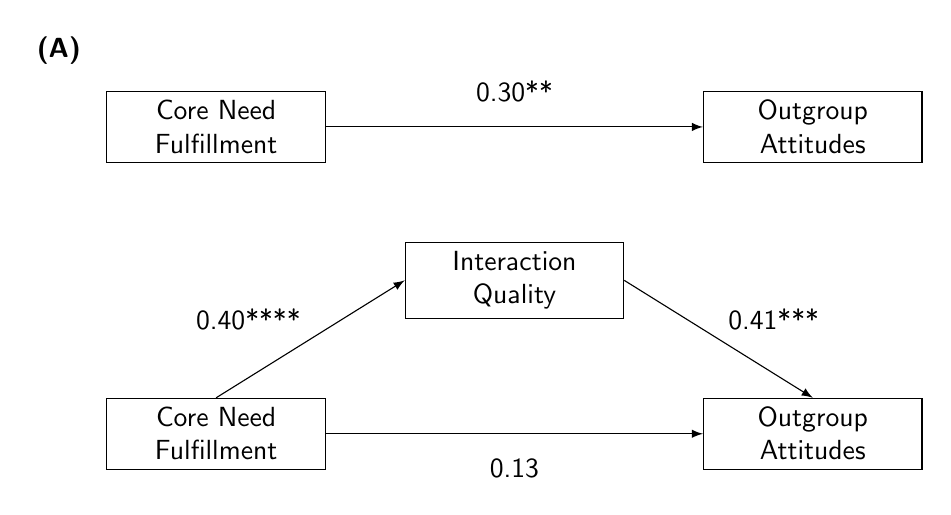
\begin{tikzpicture}[font=\sffamily]
    \node[mynode] (m){Interaction\\Quality};
    \node[mynode,below left=of m](x) {Core Need\\Fulfillment};
    \node[mynode,below right=of m](y) {Outgroup\\Attitudes};
    \node[mynode,above left=of m](xd) {Core Need\\Fulfillment};
    \node[mynode,above right=of m](yd) {Outgroup\\Attitudes};
    \draw[-latex] (xd.east) -- node[above=2mm, align=center] {0.30**} (yd.west);
    \draw[-latex] (x.north) -- node[auto] {0.40****} (m.west);
    \draw[-latex] (m.east) -- node[auto] {0.41***} (y.north);
    \draw[-latex] (x.east) -- node[below=2mm, align=center] {0.13} (y.west);
    \path (xd.north west) ++(-0.2, 6pt) node[above left]{\textbf{(A)}};
\end{tikzpicture}

\vspace{24pt}

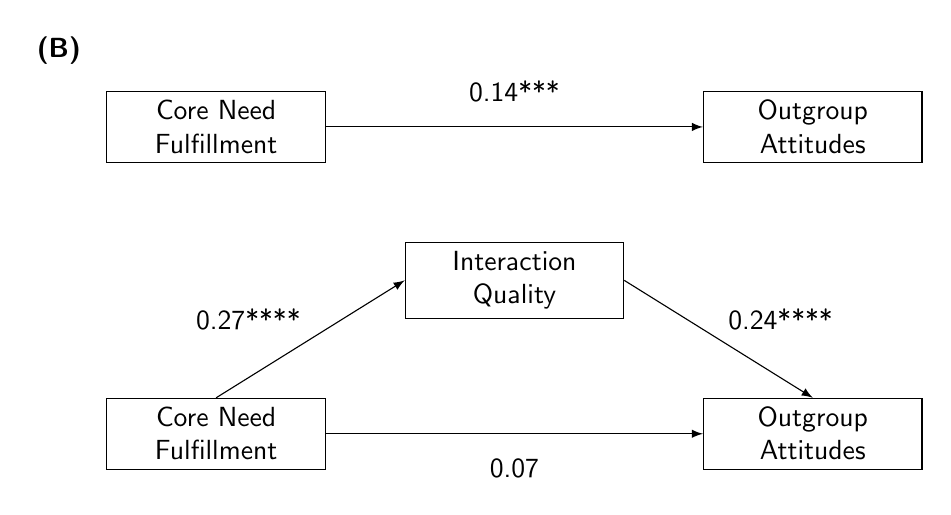
\begin{tikzpicture}[font=\sffamily]
    \node[mynode] (m){Interaction\\Quality};
    \node[mynode,below left=of m](x) {Core Need\\Fulfillment};
    \node[mynode,below right=of m](y) {Outgroup\\Attitudes};
    \node[mynode,above left=of m](xd) {Core Need\\Fulfillment};
    \node[mynode,above right=of m](yd) {Outgroup\\Attitudes};
    \draw[-latex] (xd.east) -- node[above=2mm, align=center] {0.14***} (yd.west);
    \draw[-latex] (x.north) -- node[auto] {0.27****} (m.west);
    \draw[-latex] (m.east) -- node[auto] {0.24****} (y.north);
    \draw[-latex] (x.east) -- node[below=2mm, align=center] {0.07} (y.west);
    \path (xd.north west) ++(-0.2, 6pt) node[above left]{\textbf{(B)}};
\end{tikzpicture}

\vspace{24pt}

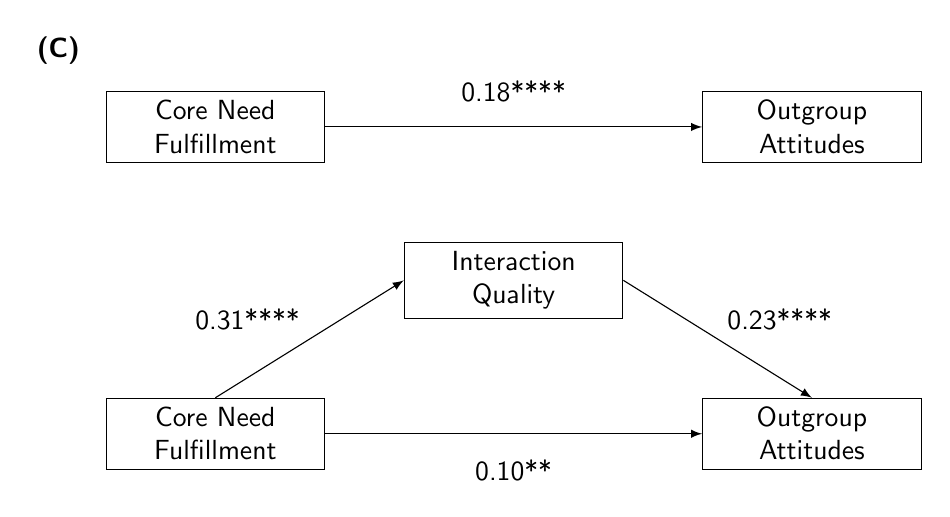
\begin{tikzpicture}[font=\sffamily]
    \node[mynode] (m){Interaction\\Quality};
    \node[mynode,below left=of m](x) {Core Need\\Fulfillment};
    \node[mynode,below right=of m](y) {Outgroup\\Attitudes};
    \node[mynode,above left=of m](xd) {Core Need\\Fulfillment};
    \node[mynode,above right=of m](yd) {Outgroup\\Attitudes};
    \draw[-latex] (xd.east) -- node[above=2mm, align=center] {0.18****} (yd.west);
    \draw[-latex] (x.north) -- node[auto] {0.31****} (m.west);
    \draw[-latex] (m.east) -- node[auto] {0.23****} (y.north);
    \draw[-latex] (x.east) -- node[below=2mm, align=center] {0.10**} (y.west);
    \path (xd.north west) ++(-0.2, 6pt) node[above left]{\textbf{(C)}};
\end{tikzpicture}

  \end{center}
  \caption*{Note: \\
  (A) Study 1; (B) Study 2; (C) Study 3.\\
  General: Path coefficients are standardized regression coefficients. Statistical significance markers are based on the unstandardized regression results (as presented in \tblref{tab:intergroupNeedsTblLong}).\\
  **** p < .0001, *** p < .001, ** p < .01, * p < .05}
\end{figure}

\begin{figure}
  \caption{Contact Hypothesis}
  \label{fig:ContactHypothesis}
  \centering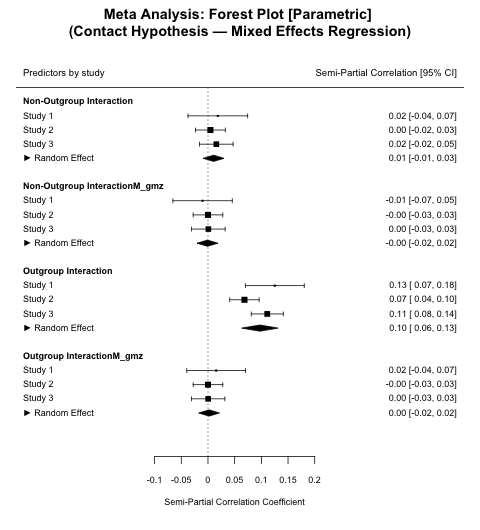
\includegraphics[width=\textwidth]{Figures/forestParametricREMLGeneralLmer.png}
  %\begin{subfigure}{\textwidth}
  %  \caption{}
  %  \centering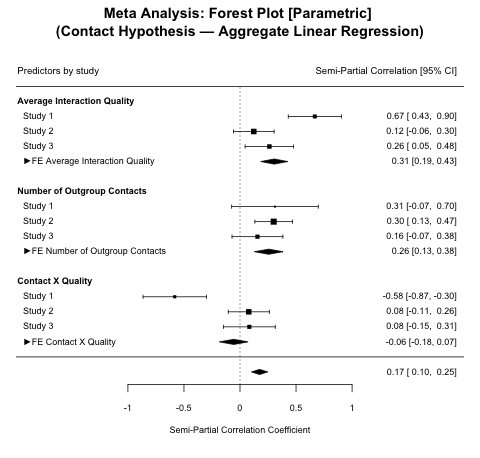
\includegraphics[width=0.75\textwidth]{Figures/forestParametricGeneralLm.png}
  %\end{subfigure}
  %\begin{subfigure}{\textwidth}
  %  \caption{}
  %  \centering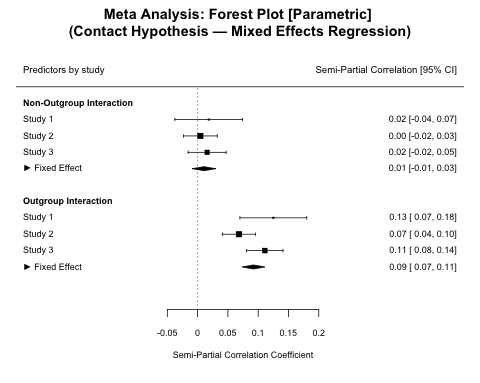
\includegraphics[width=0.75\textwidth]{Figures/forestParametricFEGeneralLmer.png}
  %\end{subfigure}
  \caption*{Note: \\
  Summary of mixed models results of the contemporaneous contact effects.\\
  General: Random effects meta analytic results are presented for completeness.}
\end{figure}

\begin{figure}
  \caption{Core Need Fulfillment}
  \label{fig:AllportNeedFulfillment}
  \centering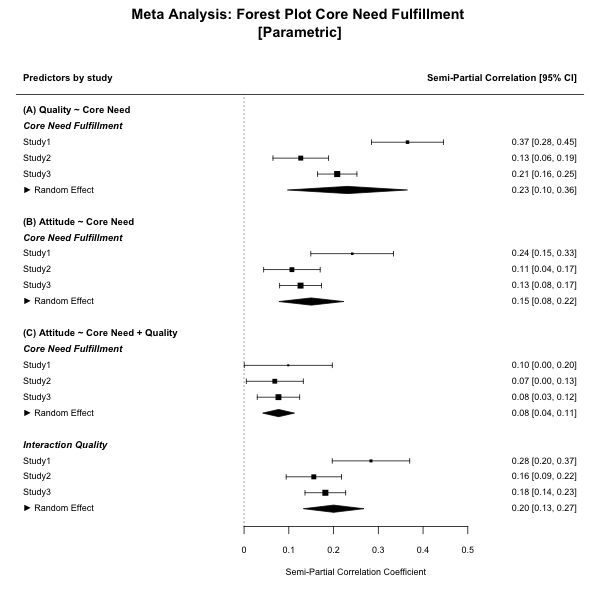
\includegraphics[width=\textwidth]{Figures/forestParametricTheoryComb.png}
  %\begin{subfigure}{\textwidth}
  %  \caption{}
  %  \centering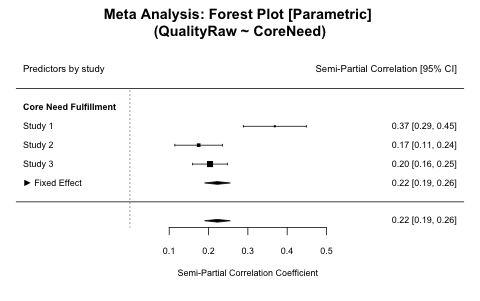
\includegraphics[width=0.6\textwidth]{Figures/forestParametricFETheoryQualityCore.png}
  %\end{subfigure}
  %\begin{subfigure}{\textwidth}
  %  \caption{}
  %  \centering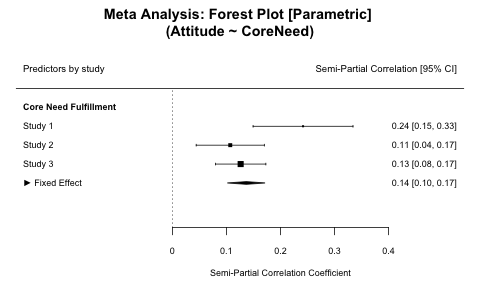
\includegraphics[width=0.6\textwidth]{Figures/forestParametricFETheoryAttitudeCore.png}
  %\end{subfigure}
  %\begin{subfigure}{\textwidth}
  %  \caption{}
  %  \centering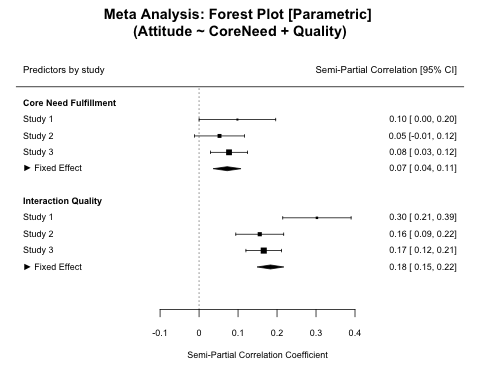
\includegraphics[width=0.6\textwidth]{Figures/forestParametricFETheoryAttitudeCoreQuality.png}
  %\end{subfigure}
  \caption*{Note: \\
  (a) Core Need Fulfillment predicting Interaction Quality.\\
  (b) Core Need Fulfillment predicting Outgroup Attitudes.\\
  (c) Core Need Fulfillment and Interaction Quality predicting Outgroup Attitudes.\\
  General: Random effects meta analytic results are presented for completeness.}
\end{figure}


\printbibliography

\appendix

\section{Hypotheses and Analysis Plan}
\label{app:AppendixHypotheses}

\newlength{\mdfmar}
\setlength{\mdfmar}{1.5em}
\mdfdefinestyle{mdfhypothesis}{
    innerleftmargin = +1.5\mdfmar, %
    innerrightmargin = +1.5\mdfmar, 
    innertopmargin = +\mdfmar, 
    innerbottommargin = +\mdfmar, 
    skipabove = 12pt
}
\newlength{\subhypskip}
\setlength{\subhypskip}{1.5em}
\newlength{\eqskip}
\setlength{\eqskip}{3.5em}

In this appendix, we present the expanded hypotheses and their associated analysis plan. Given the nested structure of much of our data we test many of our hypotheses using a multilevel approach, where $y_{ti}$ denotes the response at measurement occasion $t$ ($t = 1, ...,T_i$; level 1) for individual $i$ ($i = 1, ..., n$; level 2). All multilevel assumptions are tested as follows (e.g., for random slopes model with $j$ within-person predictors):

\begin{flalign}
  &\textrm{Level 1 Variance:}\ e_{ti} \sim \mathcal{N}(0,\sigma^2) \\
  &\textrm{Level 2 Variance:}\ \begin{bmatrix} u_{0i}\\ \vdots\\ u_{ji}\end{bmatrix} 
  \sim \mathcal{N}
  \begin{pmatrix}
    \begin{bmatrix} 
      0 \\ 
      \vdots \\
      0
    \end{bmatrix}, 
    \begin{bmatrix} 
      \tau_{00}^2 &  & \\ 
      \vdots & \ddots & \\
      \tau_{j0} & \ldots & \tau_{jj}^2
    \end{bmatrix}
  \end{pmatrix}
\end{flalign}

For our main aims we sequentially focus on four sets of models to test and validate our hypotheses:

\subsection{1. Contact hypothesis in extensive longitudinal data.} 
Within the individual studies, we begin by testing the most basic assumption of the intergroup contact hypothesis that outgroup attitudes should be more positive after outgroup interactions but not after non-outgroup interactions. For this we use multi-level regression analyses, predicting outgroup attitudes from outgroup interaction and non-outgroup interaction dummy variables. We also include the participant means as level two predictors to fully disentangle within- (level 1) and between-participant (level 2) effects of intergroup contact \citep[e.g.,][Section 4.6]{Snijders2012}.

\begin{mdframed}[style=mdfhypothesis]
    \begin{hyp}[H\ref{hyp:contactHyp}] \label{hyp:contactHyp}
        Based on the most general understanding of the contact hypothesis, positive intergroup contacts should be associated with more favorable outgroup attitudes across extensive longitudinal data.
    \end{hyp}
    
    \begin{subhyp}[H\ref{hyp:contactDummyML}] \label{hyp:contactDummyML}
    \addtolength{\leftskip}{\subhypskip}
    Outgroup attitudes should be more positive after an intergroup interaction compared to a non-outgroup interaction.
    \end{subhyp}

    \begin{fleqn}[\eqskip] 
    \begin{equation} \label{eq:ContactDummy}
      \begin{split}
        \textrm{Level 1:} &
          \begin{aligned}[t]
            \ Attitude_{ti} =  &\ \beta_{0i} + \beta_{1i}OutgroupInteraction_{ti} + \\
                               &\ \beta_{2i}NonOutgroupInteraction_{ti} + e_{ti}
          \end{aligned} \\
        \textrm{Level 2:} &
            \begin{aligned}[t]
                \ \beta_{0i} = &\ \gamma_{00} + \gamma_{01}MeanOutgroupInteraction_{i} + \\
                               &\ \gamma_{02}MeanNonOutgroupInteraction_{i} + u_{0i} \\
                  \beta_{1i} = &\ \gamma_{10} + u_{1i} \\
                  \beta_{2i} = &\ \gamma_{20} + u_{2i}
            \end{aligned}
      \end{split} 
    \end{equation}
    \end{fleqn}
\end{mdframed}

\hl{OPTION 1:} We then seek to investigate intergroup contacts and perceived interaction quality jointly. Notably, however, participants are only able to report their interaction quality perceptions if they had an interaction. This is considered to be structurally missing data and cannot meaningfully be imputed for modeling. To deal with this issue, we mimic the procedure commonly used within the cross-section literature. In particular, we conduct a person-level linear regression by aggregating the number of outgroup interactions participants had, their average interaction quality perceptions, as well as their average outgroup attitudes \citep[for possible alternative approaches see,][]{Enders2011}. To avoid an underpowered analysis, we use the aggregated data from all three studies. 
    
\hl{OPTION 2:} We then seek to test the full contact hypothesis by investigating intergroup contacts and perceived interaction quality jointly. To do so, we conduct a person-level linear regression using person-level aggregated data from all three studies. In particular, we aggregate the number of outgroup interactions participants had, their average interaction quality perceptions, as well as their average outgroup attitudes. This approach has three main benefits: (1) Interaction quality ratings are only available if participants had an interaction, and the aggregation deals with this structural missingness. (2) Using the participant-level data from all three studies, we avoid potential power issues. (3) This analysis mimics the analyses conducted within the cross-section literature, where participants are asked to recall how many interactions they had over a one-month period, how positive these interactions were, and what their general attitudes towards the outgroup are.

\begin{mdframed}[style=mdfhypothesis]
    \begin{subhyp}[H\ref{hyp:contactCor}] \label{hyp:contactCor}
    \addtolength{\leftskip}{\subhypskip}
    Participants with more intergroup interactions should have more favorable outgroup attitudes.
    \end{subhyp}

      \begin{fleqn}[\eqskip] 
        \begin{equation} \label{eq:ContactCor}
            r_{\left(ContactFrequency_{i},\ AverageQuality_{i}\right)} > 0
        \end{equation}
      \end{fleqn}

    \begin{subhyp}[H\ref{hyp:contactQualLM}] \label{hyp:contactQualLM}
    \addtolength{\leftskip}{\subhypskip}
    Participants with more intergroup interactions should have more favorable outgroup attitudes depending on the average interaction quality.
    \end{subhyp}

      \begin{fleqn}[\eqskip] 
        \begin{equation} \label{eq:contactQualLM}
            \begin{split}
              AverageAttitude_{i} = &\ \beta_{0} + \beta_{1}ContactFrequency_{i} + \\
                                    &\ \beta_{2}AverageQuality_{i} +\\
                                    &\ \beta_{3}ContactFrequency_{i} * AverageQuality_{i}
            \end{split}
        \end{equation}
      \end{fleqn}  
      
      We additionally control for the participant's study membership.
\end{mdframed}
Because this analysis uses the data from all three studies, the results of this analysis are presented in the `Robustness, Stability, and Embeddedness across Studies' section.

\subsection{2. Core need fulfillment during intergroup contact.}
The main proposal of this manuscript has been the assertion that the fulfillment of situation core needs during an interaction will be associated with more positive interaction quality perceptions and, ultimately, more positive outgroup attitudes. Thus, for the main set of analyses, we focus on the reported outgroup interactions only. For each study, we will use multi-level regressions to test the main three assertions of our proposal (mirroring the basic steps of a traditional mediation analysis).

\begin{mdframed}[style=mdfhypothesis]
    \begin{hyp}[H\ref{hyp:keyNeed}] \label{hyp:keyNeed}
    Based on our proposal, intergroup interactions with higher situational core need fulfillment should predict more favorable outgroup attitudes due to more positive interaction quality perceptions.
    \end{hyp}
    
    \setcounter{subhyp}{0}
    \begin{subhyp}[H\ref{hyp:keyNeedPred}] \label{hyp:keyNeedPred}
    \addtolength{\leftskip}{\subhypskip}
    Core need fulfillment during outgroup interactions should predict more positive outgroup attitudes.
    \end{subhyp}
    
    \begin{fleqn}[\eqskip]
      \begin{equation} \label{eq:SlopesAttCore}
        \begin{split}
            \textrm{Level 1:} &\ Attitude_{ti} = \beta_{0i} + \beta_{1i}KeyNeedFulfill_{ti} + e_{ti}\\
            \textrm{Level 2:} &\ \beta_{0i} = \gamma_{00} + u_{0i} \\
                              &\ \beta_{1i} = \gamma_{10} + u_{1i}
        \end{split}
      \end{equation}
    \end{fleqn}
    
    \begin{subhyp}[H\ref{hyp:keyNeedQual}] \label{hyp:keyNeedQual}
    \addtolength{\leftskip}{\subhypskip}
    Core need fulfillment during outgroup interactions should also predict higher perceived interaction quality.
    \end{subhyp}
    
    \begin{fleqn}[\eqskip]
      \begin{equation} \label{eq:SlopesQltCore}
        \begin{split}
            \textrm{Level 1:} &\ InteractionQuality_{ti} = \beta_{0i} + \beta_{1i}KeyNeedFulfill_{ti} + e_{ti}\\
            \textrm{Level 2:} &\ \beta_{0i} = \gamma_{00} + u_{0i} \\
                              &\ \beta_{1i} = \gamma_{10} + u_{1i}
        \end{split}
      \end{equation}
    \end{fleqn}
    
    \begin{subhyp}[H\ref{hyp:keyNeedMediation}] \label{hyp:keyNeedMediation}
    \addtolength{\leftskip}{\subhypskip}
    The effect of core need fulfillment on outgroup attitudes should be reduced when considered together with perceived interaction quality.
    \end{subhyp}
    
    \begin{fleqn}[\eqskip]
      \begin{equation} \label{eq:SlopesAttCoreQual}
        \begin{split}
          \textrm{Level 1:} &
            \begin{aligned}[t]
              \ Attitude_{ti} =  &\ \beta_{0i} + \beta_{1i}KeyNeedFulfill_{ti} + \\
                                 &\ \beta_{2i}InteractionQuality_{ti} + e_{ti}
            \end{aligned} \\
          \textrm{Level 2:} &\ \beta_{0i} = \gamma_{00} + u_{0i} \\
                            &\ \beta_{1i} = \gamma_{10} + u_{1i} \\
                            &\ \beta_{2i} = \gamma_{20} + u_{2i}
        \end{split} 
      \end{equation}
    \end{fleqn}
\end{mdframed}

\subsection{3. Allport's conditions in extensive longitudinal data.}
Within the third study, we formally measure all of Allport's optimal contact conditions. We use multi-level regression models to test whether the fulfillment of Allport's conditions in real-life data predicts more positive outgroup attitudes and higher perceived interaction quality, using the same approach as for the core need fulfillment above.

\begin{mdframed}[style=mdfhypothesis]
    \begin{hyp}[H\ref{hyp:Allport}] \label{hyp:Allport}
    Based on Allport's optimal contact conditions, intergroup interactions with equal status, common goals, collaboration, and structural support should predict more favorable outgroup attitudes due to more positive interaction quality perceptions.
    \end{hyp}
    
    \setcounter{subhyp}{0}
    \begin{subhyp}[H\ref{hyp:AttAllport}] \label{hyp:AttAllport}
    \addtolength{\leftskip}{\subhypskip}
    Higher fulfillment of Allport's conditions during outgroup interactions should predict more positive outgroup attitudes.
    \end{subhyp}
    
    \begin{fleqn}[\eqskip]
      \begin{equation} \label{eq:SlopesAttAllport}
        \begin{split}
            \textrm{Level 1:} &\ Attitude_{ti} = \beta_{0i} + \beta_{1i}Allport_{ti} + e_{ti}\\
            \textrm{Level 2:} &\ \beta_{0i} = \gamma_{00} + u_{0i} \\
                              &\ \beta_{1i} = \gamma_{10} + u_{1i}
        \end{split}
      \end{equation}
    \end{fleqn}
    
    \begin{subhyp}[H\ref{hyp:QltAllport}] \label{hyp:QltAllport}
    \addtolength{\leftskip}{\subhypskip}
    Higher fulfillment of Allport's conditions during outgroup interactions should also predict higher perceived interaction quality.
    \end{subhyp}
    
    \begin{fleqn}[\eqskip]
      \begin{equation} \label{eq:SlopesQltAllport}
        \begin{split}
            \textrm{Level 1:} &\ InteractionQuality_{ti} = \beta_{0i} + \beta_{1i}Allport_{ti} + e_{ti}\\
            \textrm{Level 2:} &\ \beta_{0i} = \gamma_{00} + u_{0i} \\
                              &\ \beta_{1i} = \gamma_{10} + u_{1i}
        \end{split}
      \end{equation}
    \end{fleqn}
    
    \begin{subhyp}[H\ref{hyp:AttAllportQual}] \label{hyp:AttAllportQual}
    \addtolength{\leftskip}{\subhypskip}
    The effect of higher fulfillment of Allport's conditions on outgroup attitudes should be reduced when considered together with perceived interaction quality.
    \end{subhyp}
    
    \begin{fleqn}[\eqskip]
      \begin{equation} \label{eq:SlopesAttAllportQual}
        \begin{split}
          \textrm{Level 1:} &
            \begin{aligned}[t]
              \ Attitude_{ti} =  &\ \beta_{0i} + \beta_{1i}Allport_{ti} + \\
                                 &\ \beta_{2i}InteractionQuality_{ti} + e_{ti}
            \end{aligned} \\
          \textrm{Level 2:} &\ \beta_{0i} = \gamma_{00} + u_{0i} \\
                            &\ \beta_{1i} = \gamma_{10} + u_{1i} \\
                            &\ \beta_{2i} = \gamma_{20} + u_{2i}
        \end{split} 
      \end{equation}
    \end{fleqn}
\end{mdframed}

We then compare the effect of Allport's contact conditions with our core need fulfillment by comparing the model fit statistics of the two individual models and by adding both concepts to a joint multi-level regression model, to see whether the two approaches explain the same variance in outgroup attitudes.

\begin{mdframed}[style=mdfhypothesis]
    \begin{hyp}[H\ref{hyp:NeedAllport}] \label{hyp:NeedAllport}
    Based on our proposal, the fulfillment of the core situational need should predict outgroup attitudes at least as well as Allport's conditions.
    \end{hyp}

    \setcounter{subhyp}{0}
    \begin{subhyp}[H\ref{hyp:compModel}] \label{hyp:compModel}
    \addtolength{\leftskip}{\subhypskip}
    The need model (H\ref{hyp:keyNeedPred}) should predict more variance in outgroup attitudes than the model based on Allport's conditions (H\ref{hyp:AttAllport}).
    \end{subhyp}

    \begin{fleqn}[\eqskip] 
        \begin{equation}
            \begin{split}
                AIC_{KeyNeedModel} & < AIC_{AllportModel} \\
                BIC_{KeyNeedModel} & < BIC_{AllportModel}
            \end{split}
        \end{equation}
    \end{fleqn}

    \begin{subhyp}[H\ref{hyp:compTogether}] \label{hyp:compTogether}
    \addtolength{\leftskip}{\subhypskip}
    The  effect of key need fulfillment on outgroup attitudes should  persist even when taking other Allport's conditions into account. Thus, the effect of key need fulfillment on outgroup attitudes should remain strong even after controlling for Allport's conditions.  
    \end{subhyp} 
    
    \begin{fleqn}[\eqskip]
      \begin{equation} \label{eq:SlopesAttCoreAllport}
        \begin{split}
          \textrm{Level 1:} &
            \begin{aligned}[t]
              \ Attitude_{ti} =  &\ \beta_{0i} + \beta_{1i}KeyNeedFulfill_{ti} + \\
                                 &\ \beta_{2i}Allport_{ti} + e_{ti}
            \end{aligned} \\
          \textrm{Level 2:} &\ \beta_{0i} = \gamma_{00} + u_{0i} \\
                            &\ \beta_{1i} = \gamma_{10} + u_{1i} \\
                            &\ \beta_{2i} = \gamma_{20} + u_{2i}
        \end{split} 
      \end{equation}
    \end{fleqn}
\end{mdframed}

\subsection{4. Robustness, stability, and embeddedness across studies}
Within the final set of analyses, we look at the broader picture of our results and leverage the data from all participants to contextualize our results.  

\paragraph{Robustness within studies}
To build further confidence in the effect of core need fulfillment during outgroup interactions, we conduct two additional robustness analyses for each study.

Firstly, to check for the role of alternate psychological needs, we add the fulfillment of self-determination theory needs (i.e., competence, autonomy, and relatedness) to the multi-level regression. We then also compare the model with models that predicts outgroup attitudes from self-determination theory need fulfillments or core need fulfillments only. 

\begin{mdframed}[style=mdfhypothesis]
    \begin{hyp}[H\ref{hyp:keyNeedSDT}] \label{hyp:keyNeedSDT}
    The effect of key need fulfillment on outgroup attitudes should persist even when taking other fundamental psychological needs into account. Thus, the effect of key need fulfillment on outgroup attitudes should remain strong even after controlling for autonomy, competence, and relatedness fulfillment during the interaction (cf., self-determination theory). 
    \end{hyp}
    
    \begin{fleqn}[\eqskip-\subhypskip]
      \begin{equation} \label{eq:SlopesAttCoreSdt}
        \begin{split}
          \textrm{Level 1:} &
            \begin{aligned}[t]
              \ Attitude_{ti} =  &\ \beta_{0i} + \beta_{1i}KeyNeedFulfill_{ti} + \beta_{2i}Autonomy_{ti} + \\
                                 &\ \beta_{3i}Competence_{ti} + \beta_{4i}Relatedness_{ti} + e_{ti}
            \end{aligned} \\
          \textrm{Level 2:} &\ \beta_{0i} = \gamma_{00} + u_{0i} \\
                            &\ \beta_{1i} = \gamma_{10} + u_{1i} \\
                            &\ \beta_{2i} = \gamma_{20} + u_{2i} \\
                            &\ \beta_{3i} = \gamma_{30} + u_{3i} \\
                            &\ \beta_{4i} = \gamma_{40} + u_{4i}
        \end{split} 
      \end{equation}
    \end{fleqn}
\end{mdframed}

To ensure that the core need fulfillment is outgroup contact specific, we return to the full sample of intensive longitudinal measurements within each study and test whether there is an interaction effect of outgroup contact (vs. no outgroup contact) and core need fulfillment. We expect that the effect of core need fulfillment is specific to outgroup interactions and not merely due to a more need-fulfilled life in general.

\begin{mdframed}[style=mdfhypothesis]
    \begin{hyp}[H\ref{hyp:keyNeedContactType}] \label{hyp:keyNeedContactType}
    \addtolength{\leftskip}{1em}
    The effect of key need fulfillment on outgroup attitudes should be specific to intergroup interactions and not be due to need fulfillment in general. Thus, the effect of key need fulfillment on outgroup attitudes should be stronger for intergroup interactions than for ingroup interactions. 
    \end{hyp}
    
    \begin{fleqn}[\eqskip-\subhypskip]
      \begin{equation} \label{eq:SlopesAttCoreXContact}
        \begin{split}
          \textrm{Level 1:} &
            \begin{aligned}[t]
              \ Attitude_{ti} =  &\ \beta_{0i} + \beta_{1i}KeyNeedFulfill_{ti} + \\
                                 &\ \beta_{2i}OutgroupInteraction_{ti} + \\
                                 &\ \beta_{3i}KeyNeedFulfill*OutgroupInteraction_{ti} + e_{ti}
            \end{aligned} \\
          \textrm{Level 2:} &\ \beta_{0i} = \gamma_{00} + u_{0i} \\
                            &\ \beta_{1i} = \gamma_{10} + u_{1i} \\
                            &\ \beta_{2i} = \gamma_{20} + u_{2i} \\
                            &\ \beta_{3i} = \gamma_{30} + u_{3i}
        \end{split} 
      \end{equation}
    \end{fleqn}
\end{mdframed}
The results of the robustness analyses are presented in \appref{app:AppendixRobustness} to allow for a more concise presentation of our main hypotheses in the main text.

\paragraph{Stability across studies}
We assess the stability of our main analyses. We use forest plots (including meta-analytical estimates) to visualize the direction and effect sizes of our three studies.

\begin{mdframed}[style=mdfhypothesis]
    \begin{hyp}[H\ref{hyp:Stability}] \label{hyp:Stability}
    \addtolength{\leftskip}{1em}
    The effects of our main hypotheses and robustness analyses should be consistent across studies.
    \end{hyp}
\end{mdframed}

\paragraph{Embeddedness of code needs}
We, finally, use the qualitative data from the participants' self-identified core needs to contextualize our results. We leverage machine learning to extract a topic model of the free-text entries across the three studies. We describe the extracted topics and themes and compare them to the need contents usually found and measured within the psychological literature. Full methodological details and visualizations are available in Supplemental Material C.

\begin{mdframed}[style=mdfhypothesis]
    \addtolength{\leftskip}{1em}
    \textit{This analysis is data-driven and exploratory. As such, the analysis has no associated hypothesis.}
\end{mdframed}



\section{Robustness Analyses}
\label{app:AppendixRobustness}

In this appendix, we present the two additional robustness analyses that we conducted within each of the three studies. These analyses are specifically designed to check for alternative need models and to check that the effect of situation core need fulfillment is contact-specific. (1) To check for the role of alternate psychological needs, we add the fulfillment of self-determination theory needs (i.e., competence, autonomy, and relatedness) to the multi-level regression. We then also compare the model with models that predicts outgroup attitudes from self-determination theory need fulfillments or core need fulfillments only. (2) To ensure that the core need fulfillment is outgroup contact specific, we return to the full sample of intensive longitudinal measurements within each study and test whether there is an interaction effect of outgroup contact (vs. no outgroup contact) and core need fulfillment. We expect that the effect of core need fulfillment is specific to outgroup interactions and not merely due to a more need-fulfilled life in general.

As with the main analyses, full surveys are available in our OSF
repository \citep{KreienkampMasked2022a} and the full data description
is available in Online Supplementary Material A. Correlations and
descriptive statistics of the included variables are available in
\tblref{tab:descrFullWide} and \tblref{tab:descrOutWide}.

\subsection{Additional Materials}

In addition to the measurement of whether or not participants had an
intergroup interaction and their situational core need fulfillment, we
also included a number of variables that allowed us to assess the
robustness of our results.

\subsubsection{Specific Psychological Needs}

In addition to the intergroup contact dummy and situational core need
reported in the main text, we included a common measure of three
self-determination theory needs \citep[see][]{Downie2008}. The
measurement was identical in all three studies. The items were
introduced either by ``\textit{During the interaction:}'' or
``\textit{This morning [/afternoon]:}'' and measured autonomy
(``\textit{I was myself.}''), competence
(``\textit{I felt competent.}''), and relatedness (without intergroup
contact ``\textit{I had a strong need to belong}''; with intergroup
contact: ``\textit{I shared information about myself.}'' and
``\textit{The other(s) shared information about themselves.}''). All
items were rated on a continuous slider scale from very little (-50) to
a great deal (+50).

\subsubsection{Interaction Intent}

To assess whether an interaction was accidental (vs.~planned), we asked
participants with a single item to report the extend to which ``The
interaction with -X- was accidental''. The respondents were asked to
report this context variable for all interactions they reported on using
a continuous slider ranging from ``not at all'' (0), through ``very
little'' (33) and ``somewhat'' (66), to ``a great deal'' (100). In all
studies the scale showed a right skew (\textit{mean} = 29.60,
\textit{sd} = 33.68).

\subsubsection{Goal-directedness}

To assess whether the need content (i.e., the motives) would impact the
effect of the need fulfillment experiences, we manually coded the topics
we extracted during the topic modeling on two dimensions of how much
they reflect a practical and a psychological goal-directedness. We chose
practical and psychological needs specifically as our dimensions to
account for differences in the types of needs that participants commonly
reported. With practical motives we refer to specific, tangible goals or
tasks that participants aimed to accomplish during the interaction.
These instrumental goals are usually observable, concrete, and often
centered on external outcomes, such as acquiring resources, completing
tasks, and addressing immediate challenges \citep[e.g.,][]{oduntan2019}.
With psychological motives we refer to underlying motives or desires
that are more abstract and relate to personal fulfillment and
well-being. In contrast to practical needs, psychological needs delve
into the subjective and internal aspects of human experiences. These
needs pertain to emotions, social connections, and cognitive processes,
reflecting individuals' quest for personal growth, well-being, and
thriving in social relationships \citep[][]{dweck2017}. Note that with
this approach any particular motive can include a practical and/or a
psychological goal-directedness but can also be classified as not having
any goal at all. The full coding protocol we developed with examples for
each of the codes is available in our Online Supplemental Material D.
After an initial training, each of the two coders independently coded
the 47 topics on the two dimensions, using one of three options each
(i.e., 0 = no goal, 1 = vague goal, 2 = clear goal). Inter-rater
reliability assessments showed that for both the practical as well as
the psychological needs, agreement was not optimal using the three
answer options (agreement practical = 0.72\%, agreement psychological =
0.78\%). However, most disagreements were, if a need was present,
whether that need was vague (1) or concrete (2). We, thus, collapsed
these two categories making the ratings binary (need absent vs.~need
present). With the simpler coding, inter-rater agreement for practical
needs (0.93\%) and the psychological need (0.96\%) were much more
reliable. Using Cohen's \(\kappa\) as our measure of inter-rater
reliability, we find that both the practical need coding
(\textit{Cohen's} \(\kappa\) = 0.80, 95\%CI{[}0.58, 1.00{]}) as well as
the psychological need coding (\textit{Cohen's} \(\kappa\) = 0.86,
95\%CI{[}0.67, 1.00{]}) were very good. We thus proceeded with this
collapsed coding. After resolving coder disagreements and merging the
codings back to the free-text responses, we found that a majority of
responses showed both a practical as well as a psychological need
(57.95\%) and only few responses had no goal at all (1.03\%) with the
remaining 41.02\% having either a practical or a psychological need only
(see Online Supplemental Material A for more detailed tables and
visualizations).

\subsubsection{Well-being}

We measured experienced well-being using a visual analog scale adapted
from \citet{davies2022}. Participants were asked to respond to the the
question ``How do you feel right now?'' using a continuous visual slider
ranging from ``very sad''(-100) to ``very happy'' (100). The well-being
ratings were generally normally distributed (\textit{mean} = 64.80,
\textit{sd} = 19.25).

\subsection{Results}

To build further confidence in our results, we assessed a number of
additional models that might offer alternative explanations. We will
discuss the results in sequential order --- in every case first
considering the a global test of the model across the three studies and
only then assessing whether the global three-level regression model
suppresses any important person-level variations within the studies.

\subsubsection{Contact specific}

We begin our robustness analysis by testing whether the effect of core
need fulfillment is specific to an actual outgroup contact, rather than
need fulfillment in general. For this, we analyzed the generalized
situational core need fulfillment (either during a contact or about the
daytime in general) and tested whether the effect differed during
experience sampling measurements with and without outgroup contacts. We
start this test by assessing the effect across all three studies, using
a three-level hierarchical model, where measurements are nested within
participants, and participants are nested within studies. In this
overall model, we found no main effect of core need fulfillment (random
slopes model, grand-mean standardized to account for all levels of
variance; \textit{b} = 0.62, \textit{t}( 3.187) = 2.89, \textit{p} =
0.058, \textit{95\%CI}{[} 0.20, 1.03{]}) but a significant interaction
effect of core need fulfillment and outgroup contact (\textit{b} = 2.44,
\textit{t}(4,663.172) = 8.62, \textit{p} \textless{} .001,
\textit{95\%CI}{[} 1.89, 3.00{]}; also see
\tblref{tab:robustnessTblLong}). While the three-level hierarchical
model can be sensitive to scaling issues, this already indicates that it
is not key need fulfillment in general --- but only key need fulfillment
during an outgroup contact that predicts more positive outgroup
attitudes.

To ensure that the results are not affected by scaling issues (e.g.,
study-level variances suppressing person-level variances) or a similar
Simpson's paradox, we additionally assess the model within each of the
three studies. Within each of the three studies, the effects are more
pronounced, so that we also see a significant effect of core need
fulfillment (all \textit{b} \textgreater{} 0.06, all \textit{p}
\textless{} 0.005) as well as outgroup contact itself (all
\textbar{}\textit{b}\textbar{} \textgreater{} 1.81, all \textit{p}
\textless{} 0.034) but the interaction effect consistently remains the
most reliable predictor of outgroup attitudes (all
\textbar{}\textit{b}\textbar{} \textgreater{} 0.06, all \textit{p}
\textless{} 0.002, also see \tblref{tab:robustnessTblLong}). There is
thus consistent evidence that need fulfillment relates to outgroup
attitudes for outgroup contacts in particular but not need fulfillment
in general.

\subsubsection{Interaction intent}

Secondly, to assess whether the need fulfillment mechanism affected by
whether the interaction was accidental or planned we ran an exploratory
moderation analysis using the participants' ratings of how much they
perceived the interaction as `accidental'. It should be noted that we
asked our participants to focus on most the important interaction (i.e.,
``\textit{The following questions will be about the interaction \underline{you consider most significant}.}'';
emphasis as in original). We again start our analysis approach by
assessing the model across all three studies, using a three-level
hierarchical model. In this overall model, we retain the main effect of
core need fulfillment (random slopes model, grand-mean standardized to
account for all levels of variance; \textit{b} = 2.87, \textit{t}(
7.979) = 7.32, \textit{p} \textless{} .001, \textit{95\%CI}{[} 2.10,
3.64{]}) but neither contact intent nor the moderation effect affect the
results (all \textbar{}\textit{b}\textbar{} \textless{} 0.27 and all
\textit{p} \textgreater{} 0.225; see \tblref{tab:robustnessTblLong} for
full results).

We again sought to ensure that the results were not affected by scaling
issues by additionally assessing the interaction intentionality model
within each of the three studies. Within each of the three studies, the
effect of core need fulfillment became even clearer (all
\textbar{}\textit{b}\textbar{} \textgreater{} 0.13, all \textit{p}
\textless{} 0.006). But in none of the studies neither outgroup contact
intention nor the moderation effect explained a significant amount of
variance in outgroup attitudes (all \textbar{}\textit{b}\textbar{}
\textless{} 0.03 and all \textit{p} \textgreater{} 0.073; also see
\tblref{tab:robustnessTblLong}). There is thus consistent evidence that
need fulfillment is related to outgroup attitudes, even when taking the
intentionality of the interaction into account --- at least in our three
samples and with a focus on the most significant interactions.

\subsubsection{Well-being outcome}

Thirdly, to build a stronger case for the relevance of need fulfillment
to minority group members, we exploratorily assessed the effect of need
fulfilling outgroup interactions on self-reported well-being. We, thus,
re-ran our main analysis but substituted the outgroup attitudes outcome
with situational well-being. As with the previous robustness analyses,
we begin with a global three-level hierarchical model (across the three
studies). We find that need fulfillment during outgroup contacts,
indeed, has a similar effect on experienced well-being (random slopes
model, grand-mean standardized to account for all levels of variance;
\textit{b} = 3.50, \textit{t}(4.219) = 6.33, \textit{p} = 0.003,
\textit{95\%CI}{[} 2.42, 4.58{]}). We found the same result when we
assessed each of the three studies individually. In each of the studies
situational need fulfillment during the outgroup interaction was related
with higher well-being ratings by the participants (random slopes model,
centered within participants; all \textbar{}\textit{b}\textbar{}
\textgreater{} 0.10, all \textit{p} \textless{} 0.009). We, thus, find
consistent and meaningful evidence that need fulfilling outgroup
interactions also relate to higher everyday well-being.

\subsubsection{Need types}

Fourthly, to assess the role of different types of motives reported by
our participants, we added our coding of practical and psychological
goal-directedness as additional predictors to our base model. We thus
had core need fulfillment predicting outgroup attitudes while also
accounting for whether the reported motives were capturing practical
and/or psychological motives. We again ran a global model, across the
three studies first. We found that core need fulfillment remain a core
predictor of outgroup attitudes (random slopes model, grand-mean
standardized to account for all levels of variance; \textit{b} = 2.27,
\textit{t}( 48.194) = 2.72, \textit{p} = 0.009, \textit{95\%CI}{[} 0.63,
3.90{]}), even after accounting for different types of motives. None of
the motive types nor the moderation effects reached statistical
significance within the overall analysis (all
\textbar{}\textit{b}\textbar{} \textless{} 1.45 and all \textit{p}
\textgreater{} 0.073; see \tblref{tab:robustnessTblLong} for full
results).

When looking at the individual studies, we again saw that the effect of
core need fulfillment remained the on only clear effect (all
\textbar{}\textit{b}\textbar{} \textgreater{} 0.14, all \textit{p}
\textless{} 0.015). Additionally, in none of the studies neither motive
type dummies nor the moderation effect explained a significant amount of
variance in outgroup attitudes (all \textbar{}\textit{b}\textbar{}
\textless{} 1.53 and all \textit{p} \textgreater{} 0.144; also see
\tblref{tab:robustnessTblLong}). We, thus, find consistent evidence that
need fulfillment is related to outgroup attitudes, even when taking the
type of need into account --- at least in our three samples.

\subsubsection{Specific psychological needs}

In a final step, we checked whether during the interaction the core
situational need remains a meaningful predictor even when taking other
fundamental psychological needs into account. We again take a two-step
approach, starting with cross-study global three-level test and then
assessing the effects within the individual studies. Within the overall
model we find that across the studies core need fulfillment remained a
strong predictor of outgroup attitudes, even after controlling for the
three self-determination theory need (random slopes model, grand-mean
standardized to account for all levels of variance; \textit{b} = 1.88,
\textit{t}(2.702) = 4.75, \textit{p} = 0.022, \textit{95\%CI}{[} 1.11,
2.66{]}). Within this overall analysis, none of the self-determination
theory needs independently predicted outgroup attitudes to a
statistically significant extent (all \textit{p} \textgreater{} 0.093).
However, some of the effect sizes were largely comparable to that of the
core need fulfillment (all \textbar{}\textit{b}\textbar{} \textless{}
2.10, particularly that of relatedness fulfillment; see
\tblref{tab:robustnessTblLong} for full results).

When looking at the individual studies, we again saw that core need
fulfillment remained a consistent predictor of outgroup attitudes, even
after accounting for the self-determination theory need (all
\textbar{}\textit{b}\textbar{} \textgreater{} 0.06, all \textit{p}
\textless{} 0.030). However, across all three studies the fulfillment of
relatedness motives also emerged as a consistent predictor of outgroup
attitudes (all \textbar{}\textit{b}\textbar{} \textgreater{} 0.06, all
\textit{p} \textless{} 0.001). Additionally, in the larger studies 2 and
3 competence fulfillment was also related to more positive outgroup
attitudes (study 2: \textit{b} = 0.05, \textit{t}(841.8) = 2.43,
\textit{p} = 0.015, \textit{95\%CI}{[} 0.01, 0.10{]}, study 3:
\textit{b} = 0.06, \textit{t}(30.20) = 2.62, \textit{p} = 0.013,
\textit{95\%CI}{[} 0.01, 0.10{]}). None of the autonomy fulfillment
effects reached statistical significance nor did the competence
fulfillment during study 1 (see \tblref{tab:robustnessTblLong} for the
full results). In short, find that across our samples, relatedness
fulfillment (and to a smaller extend competence fulfillment) are
instrumental in understanding when an outgroup contact leads to more
positive outgroup attitudes. Importantly, even when considering these
effects situational core need fulfillment remains a strong and
consistent predictor of outgroup attitudes. In some cases, we even find
that core need fulfillment takes on some of the variance that would
otherwise be explained by the self-determination theory needs (see
Online Supplemental Material A).



\subsection{Stability and Conclusion}
As with the main analyses, we use a forest plot and the associated meta-analytic estimates to assess the stability of the results across the three studies. The forest plot shows that the core need fulfillment is also consistently outgroup contact specific (\fgrref[-A]{fig:Robustness}) and remains a meaningful predictor of outgroup attitudes even when controlling for traditional psychological need fulfillments (Figure \fgrref[-B]{fig:Robustness}). In sum, we thus find that across all three studies, psychological need fulfillment remained a robust and flexible predictor of positive outgroup attitudes.

\begin{table}
\begin{minipage}[t][\textheight][t]{\textwidth}

\caption{\label{tab:robustnessTblLong}Robustness Analyses}
\centering
\resizebox{\linewidth}{!}{
\begin{tabular}[t]{lcccccccc}
\toprule
\multicolumn{1}{c}{ } & \multicolumn{2}{c}{Overall} & \multicolumn{2}{c}{Study 1} & \multicolumn{2}{c}{Study 2} & \multicolumn{2}{c}{Study 3} \\
\cmidrule(l{3pt}r{3pt}){2-3} \cmidrule(l{3pt}r{3pt}){4-5} \cmidrule(l{3pt}r{3pt}){6-7} \cmidrule(l{3pt}r{3pt}){8-9}
 & $B$ & $\beta$ & $B$ & $\beta$ & $B$ & $\beta$ & $B$ & $\beta$\\
\midrule
\addlinespace[0.3em]
\multicolumn{9}{l}{\textbf{Contact specific}}\\
\hspace{1em}(Intercept) & 65.76** [ 49.86, 72.04] &  & 71.60**** [66.33, 76.86] &  & 68.22**** [64.95, 71.49] &  & 65.17**** [62.00, 68.34] & \\
\hspace{1em}CoreNeed & 0.62 [-13.92, 14.10] & 0.01 [-0.44, 0.45] & 0.09** [ 0.04,  0.14] & 0.21 [0.13, 0.28] & 0.06**** [ 0.04,  0.08] & 0.13 [0.08, 0.17] & 0.11**** [ 0.08,  0.14] & 0.13 [0.09, 0.17]\\
\hspace{1em}OutgroupInteraction & 3.59 [-20.13,  7.99] & -0.60 [-1.74, 0.53] & 1.81* [ 0.25,  3.37] & 0.28 [0.05, 0.50] & 2.88*** [ 1.35,  4.40] & 0.23 [0.16, 0.31] & 5.41**** [ 3.72,  7.10] & 0.37 [0.27, 0.48]\\
\hspace{1em}CoreNeed:OutgroupInteraction & 2.44**** [  0.09,  0.14] & 0.01 [ 0.01, 0.01] & 0.13**** [ 0.07,  0.18] & 0.32 [0.19, 0.45] & 0.06** [ 0.02,  0.10] & 0.14 [0.06, 0.22] & 0.17**** [ 0.12,  0.21] & 0.19 [0.12, 0.26]\\
\hspace{1em}$R^2_{marginal}$ / $R^2_{conditional}$ & 0.000 / 1.000 &  & 0.017 / 0.727 &  & 0.005 / 0.818 &  & 0.037 / 0.712 & \\
\addlinespace[0.3em]
\multicolumn{9}{l}{\textbf{Interaction Intent}}\\
\hspace{1em}(Intercept) & 70.14**** [42.53, 65.97] &  & 71.43**** [65.57, 77.29] &  & 70.40**** [67.36, 73.45] &  & 68.16**** [64.95, 71.36] & \\
\hspace{1em}CoreNeed & 2.87**** [-8.58,  8.95] & 0.02 [-1.22, 1.25] & 0.17** [ 0.06,  0.29] & 0.42 [ 0.26, 0.58] & 0.13*** [ 0.07,  0.20] & 0.25 [ 0.12, 0.37] & 0.19**** [ 0.12,  0.26] & 0.24 [ 0.15, 0.32]\\
\hspace{1em}InteractionAccidental & 0.12 [-9.82,  9.92] & 0.00 [-1.07, 1.07] & 0.03 [ 0.00,  0.06] & 0.13 [ 0.02, 0.24] & 0.01 [-0.02,  0.03] & -0.02 [-0.09, 0.05] & -0.01 [-0.04,  0.01] & -0.02 [-0.08, 0.03]\\
\hspace{1em}CoreNeed:InteractionAccidental & -0.27 [ 0.00,  0.00] & 0.00 [ 0.00, 0.00] & 0.00 [ 0.00,  0.00] & 0.00 [-0.11, 0.11] & 0.00 [ 0.00,  0.00] & -0.01 [-0.08, 0.07] & 0.00 [ 0.00,  0.00] & -0.04 [-0.09, 0.02]\\
\hspace{1em}$R^2_{marginal}$ / $R^2_{conditional}$ & 0.000 / 1.000 &  & 0.135 / NA &  & 0.015 / 0.728 &  & 0.021 / 0.687 & \\
\addlinespace[0.3em]
\multicolumn{9}{l}{\textbf{Well-being Outcome}}\\
\hspace{1em}(Intercept) & 65.25*** [ 28.58, 63.85] &  & 61.34**** [55.56, 67.12] &  & 67.18**** [64.66, 69.70] &  & 63.63**** [60.85, 66.41] & \\
\hspace{1em}CoreNeed & 3.50** [-16.18, 16.62] & 0.01 [-1.33, 1.35] & 0.25** [ 0.10,  0.40] & 0.31 [0.17, 0.46] & 0.10** [ 0.04,  0.16] & 0.17 [0.11, 0.23] & 0.20*** [ 0.11,  0.29] & 0.17 [0.10, 0.25]\\
\hspace{1em}$R^2_{marginal}$ / $R^2_{conditional}$ & 0.000 / 1.000 &  & 0.054 / 0.541 &  & 0.008 / 0.348 &  & 0.017 / 0.375 & \\
\addlinespace[0.3em]
\multicolumn{9}{l}{\textbf{Need Type}}\\
\hspace{1em}(Intercept) & 69.40**** [50.54, 64.07] &  & 73.09**** [66.87, 79.31] &  & 70.37**** [67.24, 73.51] &  & 68.18**** [64.77, 71.60] & \\
\hspace{1em}CoreNeed & 2.27** [ 0.09,  0.21] & 0.01 [-0.82, 0.84] & 0.14* [ 0.03,  0.26] & 0.29 [ 0.12, 0.46] & 0.14** [ 0.06,  0.21] & 0.15 [ 0.04, 0.26] & 0.19*** [ 0.08,  0.29] & 0.18 [ 0.08, 0.29]\\
\hspace{1em}practical need & 0.01 [-4.82,  7.25] & -0.11 [-1.00, 0.78] & -0.04 [-2.76,  2.69] & -0.06 [-0.33, 0.20] & 0.80 [-1.22,  2.82] & 0.17 [ 0.01, 0.32] & -0.99 [-2.85,  0.86] & -0.02 [-0.16, 0.12]\\
\hspace{1em}psychological need & 1.45 [-8.48,  4.45] & -0.13 [-1.11, 0.84] & 1.53 [-3.66,  6.73] & 0.08 [-0.28, 0.43] & 1.50 [-0.98,  3.98] & 0.13 [-0.03, 0.30] & 1.25 [-0.42,  2.93] & 0.10 [-0.04, 0.24]\\
\hspace{1em}CoreNeed:practical need & -0.23 [-0.08,  0.05] & 0.00 [ 0.00, 0.01] & 0.01 [-0.13,  0.15] & -0.12 [-0.36, 0.12] & -0.02 [-0.15,  0.10] & -0.04 [-0.23, 0.14] & -0.05 [-0.18,  0.08] & 0.03 [-0.11, 0.18]\\
\hspace{1em}CoreNeed:psychological need & 0.67 [-0.03,  0.11] & 0.00 [ 0.00, 0.01] & -0.10 [-0.31,  0.11] & -0.02 [-0.33, 0.29] & 0.04 [-0.07,  0.15] & 0.04 [-0.13, 0.21] & 0.04 [-0.11,  0.19] & -0.06 [-0.22, 0.10]\\
\hspace{1em}$R^2_{marginal}$ / $R^2_{conditional}$ & 0.078 / NA &  & 0.046 / NA &  & 0.017 / 0.760 &  & 0.018 / 0.696 & \\
\addlinespace[0.3em]
\multicolumn{9}{l}{\textbf{Specific Psychological Needs}}\\
\hspace{1em}(Intercept) & 70.93** [41.14, 58.40] &  & 71.54**** [65.79, 77.28] &  & 70.75**** [67.59, 73.90] &  & 68.68**** [65.53, 71.82] & \\
\hspace{1em}CoreNeed & 1.88* [-5.45,  5.68] & 0.01 [-1.13, 1.15] & 0.10* [ 0.02,  0.18] & 0.27 [ 0.11, 0.43] & 0.06** [ 0.02,  0.10] & 0.14 [ 0.06, 0.22] & 0.14*** [ 0.07,  0.21] & 0.18 [ 0.09, 0.26]\\
\hspace{1em}Autonomy & 0.78 [-8.61,  8.70] & 0.01 [-1.15, 1.16] & 0.05 [-0.12,  0.23] & 0.12 [-0.02, 0.26] & 0.04 [-0.01,  0.09] & 0.05 [-0.03, 0.13] & 0.04 [ 0.00,  0.08] & 0.05 [-0.03, 0.12]\\
\hspace{1em}Competence & 0.95 [-3.70,  3.78] & 0.00 [-1.11, 1.11] & 0.05 [-0.16,  0.26] & 0.02 [-0.21, 0.25] & 0.05* [ 0.01,  0.10] & 0.06 [-0.03, 0.15] & 0.06* [ 0.01,  0.10] & 0.09 [ 0.02, 0.16]\\
\hspace{1em}Relatednesss & 2.10 [-4.04,  4.19] & 0.01 [-1.20, 1.22] & 0.10*** [ 0.06,  0.14] & 0.29 [ 0.17, 0.41] & 0.06**** [ 0.03,  0.09] & 0.16 [ 0.09, 0.24] & 0.06*** [ 0.02,  0.09] & 0.10 [ 0.02, 0.19]\\
\hspace{1em}$R^2_{marginal}$ / $R^2_{conditional}$ & 0.176 / NA &  & 0.061 / 0.860 &  & 0.025 / 0.747 &  & 0.041 / 0.702 & \\
\bottomrule
\multicolumn{9}{l}{\rule{0pt}{1em}\textit{Note: }}\\
\multicolumn{9}{l}{\rule{0pt}{1em}**** $p$ < .0001, *** $p$ < .001, ** $p$ < .01, * $p$ < .05}\\
\end{tabular}}
\end{minipage}
\end{table}


\begin{figure}
  \caption{Robustness Analyses}
  \label{fig:Robustness}
  \centering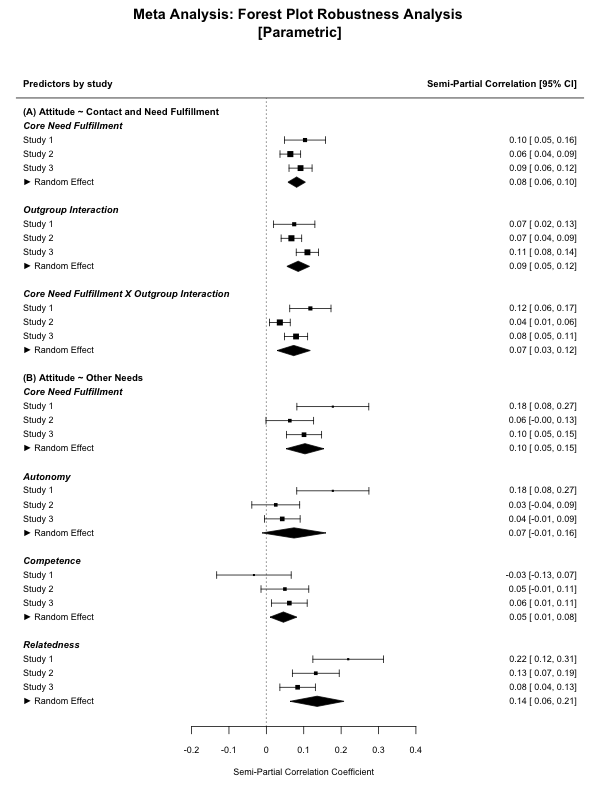
\includegraphics[width=\textwidth]{Figures/forestParametricRobustnessComb.png}
  %\begin{subfigure}{\textwidth}
  %  \caption{}
  %  \centering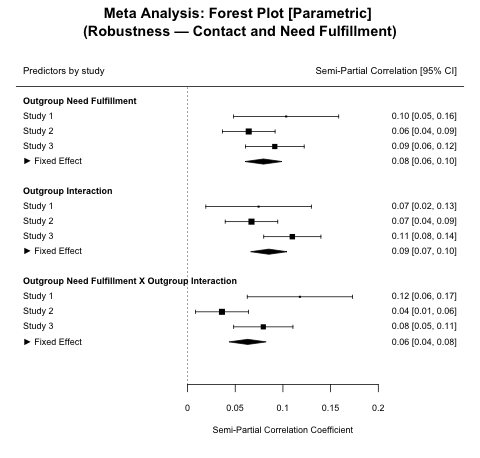
\includegraphics[width=0.65\textwidth]{Figures/forestParametricFERobustContact.png}
  %\end{subfigure}
  %\begin{subfigure}{\textwidth}
  %  \caption{}
  %  \centering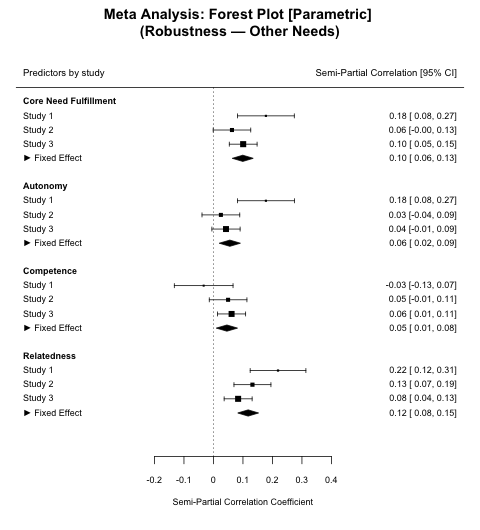
\includegraphics[width=0.65\textwidth]{Figures/forestParametricFERobustSDT.png}
  %\end{subfigure}
  \caption*{Note: \\
  (a) Need Fulfillment and Intergroup Contact predicting Outgroup Attitudes (full sample).\\
  (b) Core Need Fulfillment predicting Outgroup Attitudes while controlling for self-determination theory needs (intergroup contact sample).\\
  General: Random effects meta-analytic results are presented for completeness.}
\end{figure}


\end{document}
